\newcommand{\rmsn}{\mathrm{rms}_{90}}
%%\renewcommand{\vec}[1]{\overrightarrow{\rm{#1}}}

%%%%%%%%%%%%%%%%%%%%%%%%%%%%%%%%%%%%%%%%%%%%%%%%%%%%%%%%%%%%%%%
\subsection{Tracking}\label{sec:performance:tracking}

The efficient identification and precise reconstruction of charged particle
tracks is crucial for the overall physics performance of the ILD detector.
The goal for the asymptotic momentum resolution~\cite{ild:bib:perfgoal::barklow} is
\begin{equation*}
\sigma_{1/p_T} \approx 2\times 10^{-5}~\text{GeV}^{-1}.
\end{equation*}
ensuring that the Higgs mass measurement from $\Pep\Pem \rightarrow H, Z\rightarrow\Pmuon\APmuon$ events
is dominated by the beam energy spread rather than the detector resolution.
%%The performance goal for the  impact parameter resolution is
%%\begin{equation}
%%\sigma_{r\phi} = \unit{5}{\micron} \oplus \frac{10}{p/\unit{GeV}\sin^{3/2}\theta}~\micron
%%\end{equation}
%%crucial for the flavour tagging performance,

To evaluate the tracking resolution of the ILD detector models, samples of single $\Pmu$-events at fixed
momenta (p=\unit{1,3,5,10,15,30,100}{\GeV} ) and polar angles ($\theta=10,20,40,85^\circ$) have been
run through the full simulation and reconstruction as described in
sections~\ref{sec:det-sim} and~\ref{sec:reco} with the single point resolutions given in table~\ref{tab:ild_trk_res}.
Fig.~\ref{fig:perf:trkres} shows the results for the inverse transverse momentum resolution
$\sigma_{1/p_T}$ and the impact parameter resolutions $\sigma_{d0}$ and $\sigma_{Z0}$ in the 
$r\phi$-plane and along the $z$-axis respectively for the large and small detector models ILD-L and ILD-S.
The performance goal for the asymptotic momentum resolution is met by both detector modes as can be seen in
Fig.~\ref{fig:perf:trk_pt}. Fig.~\ref{fig:perf:trk_ptcmp} shows the ratio of the resolution for the small
and large detector. In the barrel region the larger detector is slightly better, due to the larger number of hits and
the corresponding larger lever arm, despite the lower B-field. In the forward region this behaviour
is reversed as here the same number of hits are available due to the identical detector geometry in this region
and it is the higher B-field that causes a better measurement of the curvature and thus the momentum.
The impact parameter resolutions for the large and small detector models are equal to within a few percent,
as can be seen from Fig.~\ref{fig:perf:trk_d0cmp} and~\ref{fig:perf:trk_z0cmp}, except at low momenta in the
forward region, where the large detector is better.
In the barrel region, one observes very similar resolutions for the impact parameter in the $r\phi$-plane
and that along the $z$-axis, whereas in the forward region, where less VTX-hits contribute, $\sigma_{Z0}$
is significantly worse than  $\sigma_{d0}$ (see Fig.~\ref{fig:perf:trk_d0} and~\ref{fig:perf:trk_z0})
%
% tracking resolution for single muons
% 
\begin{figure}[htbp]
\begin{subfigure}{0.49\hsize} 
 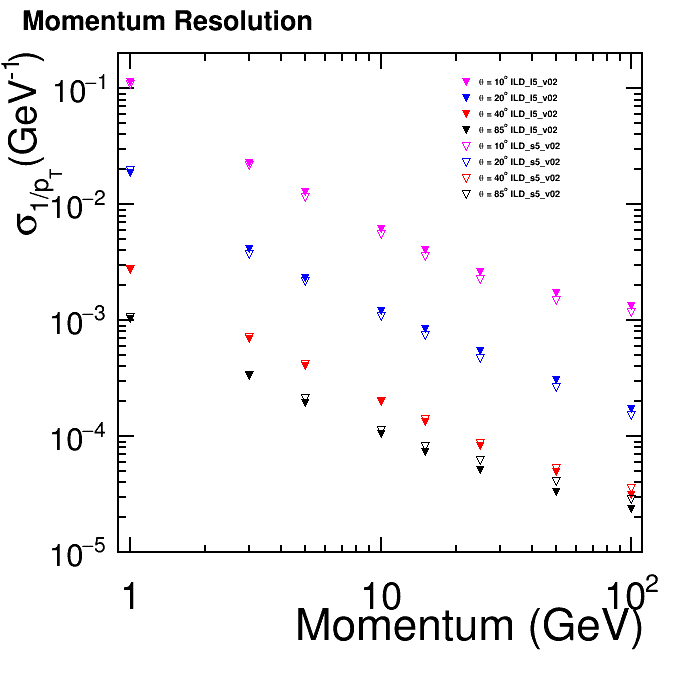
\includegraphics[width=\hsize]{Performance/fig/PResolution_compare_v02-00-02_New_ILD_ls5_v02.png}
 \caption{ \label{fig:perf:trk_pt}}
 \end{subfigure}
\begin{subfigure}{0.49\hsize} 
 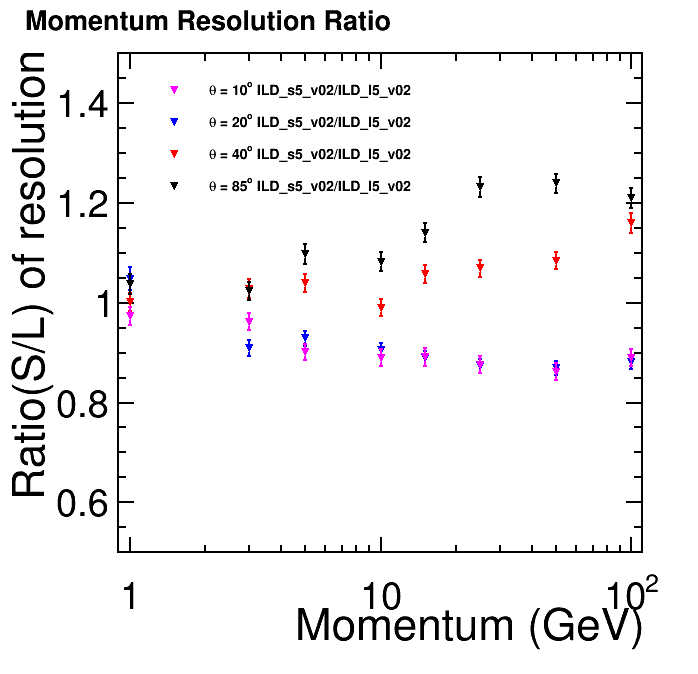
\includegraphics[width=\hsize]{Performance/fig/PResolution_Ratio_v02-00-02_New_ILD_ls5_v02.png}
 \caption{  \label{fig:perf:trk_ptcmp}}
 \end{subfigure}
\begin{subfigure}{0.49\hsize} 
 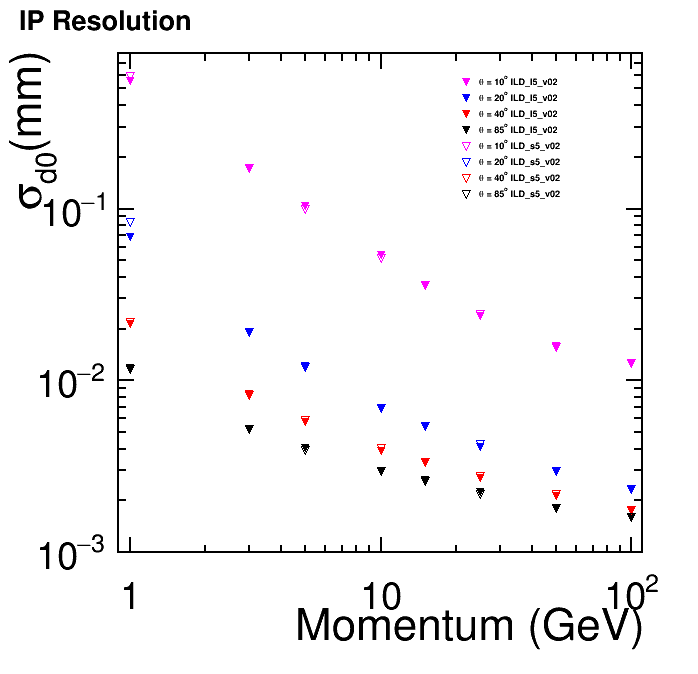
\includegraphics[width=\hsize]{Performance/fig/D0Resolution_compare_v02-00-02_New_ILD_ls5_v02.png}
 \caption{ \label{fig:perf:trk_d0}}
 \end{subfigure}
\begin{subfigure}{0.49\hsize} 
 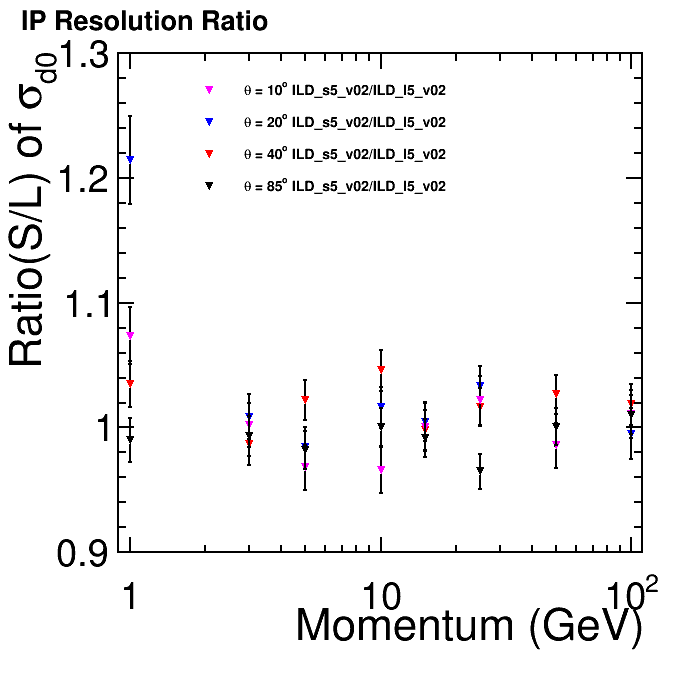
\includegraphics[width=\hsize]{Performance/fig/D0Resolution_Ratio_v02-00-02_New_ILD_ls5_v02.png}
 \caption{  \label{fig:perf:trk_d0cmp}}
 \end{subfigure}
\begin{subfigure}{0.49\hsize} 
 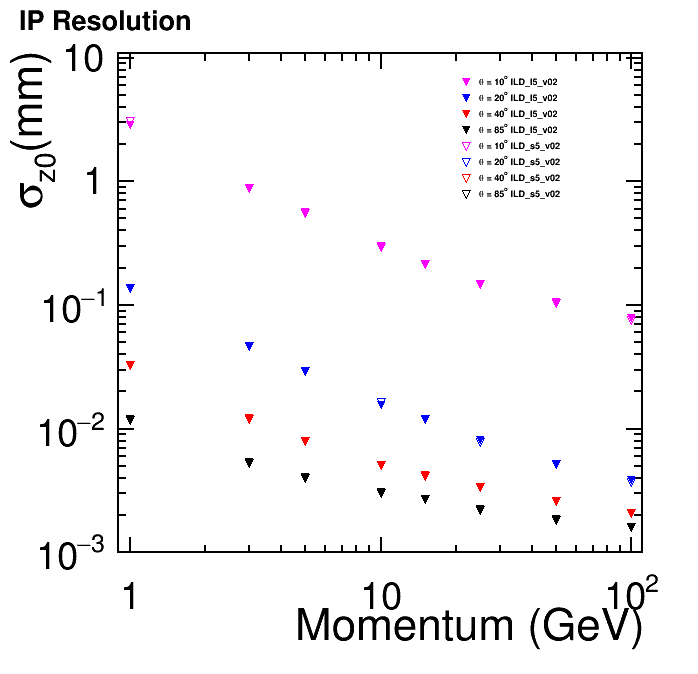
\includegraphics[width=\hsize]{Performance/fig/Z0Resolution_compare_v02-00-02_New_ILD_ls5_v02.png}
 \caption{ \label{fig:perf:trk_z0}}
 \end{subfigure}
\begin{subfigure}{0.49\hsize} 
 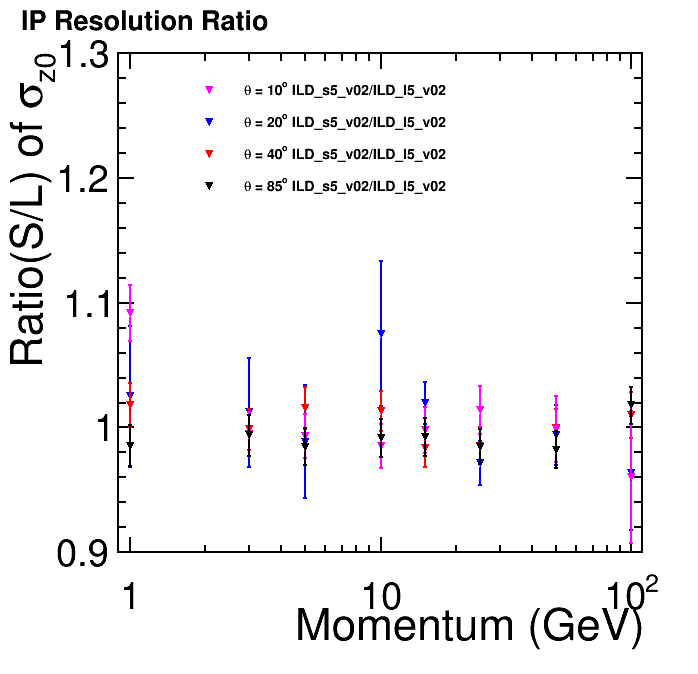
\includegraphics[width=\hsize]{Performance/fig/Z0Resolution_Ratio_v02-00-02_New_ILD_ls5_v02.png}
 \caption{  \label{fig:perf:trk_z0cmp}}
 \end{subfigure}
\caption{
  Tracking resolutions for single muons for the large and small ILD detector models.
  (a) Inverse transverse momentum resolution $\sigma_{1/p_T}$ as a function of momentum and the ratio $small/large$ in (b).
  (c) Impact parameter in the $r\phi$-plane $\sigma_{d0}$ as a function of momentum and the ratio $small/large$ in (d).
  (e) Impact parameter along the $z$-axis $\sigma_{z0}$  as a function of momentum and the ratio $small/large$  in (f).
}
\label{fig:perf:trkres}
\end{figure}

%
% % tracking efficiency for ttbar events
% 
\begin{figure}[htbp]
\begin{subfigure}{0.49\hsize} 
 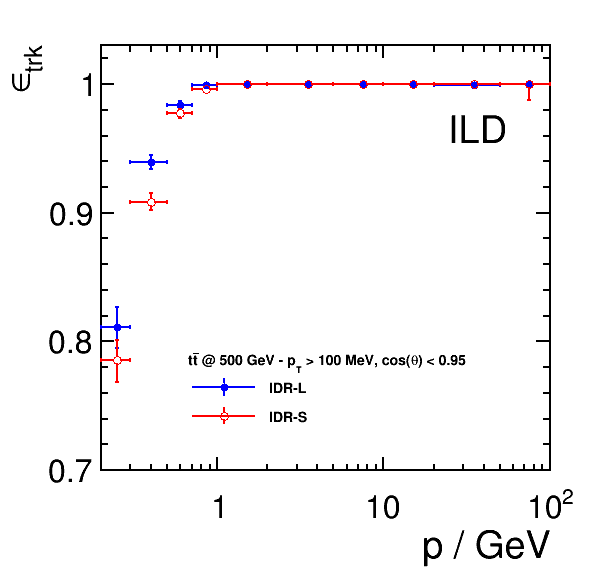
\includegraphics[width=\hsize]{Performance/fig/trkEff_p_ttbar_IDR.png}
 \caption{ \label{fig:perf:trkeff_p}}
 \end{subfigure}
\begin{subfigure}{0.49\hsize} 
 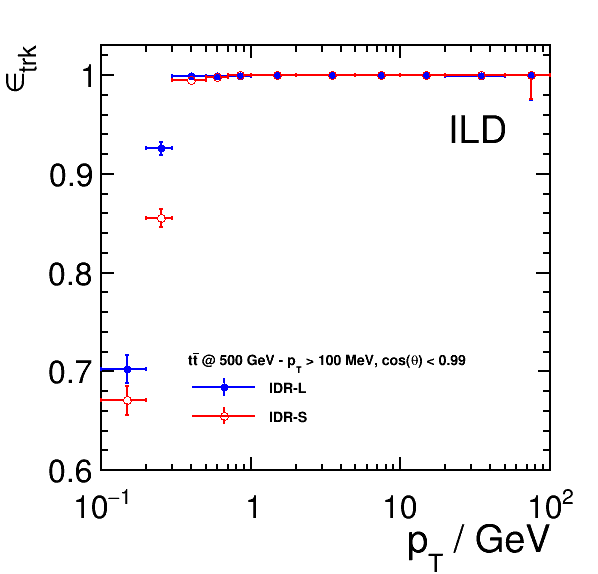
\includegraphics[width=\hsize]{Performance/fig/trkEff_pt_ttbar_IDR.png}
 \caption{  \label{fig:perf:trkeff_pt}}
 \end{subfigure}
\begin{subfigure}{0.49\hsize} 
 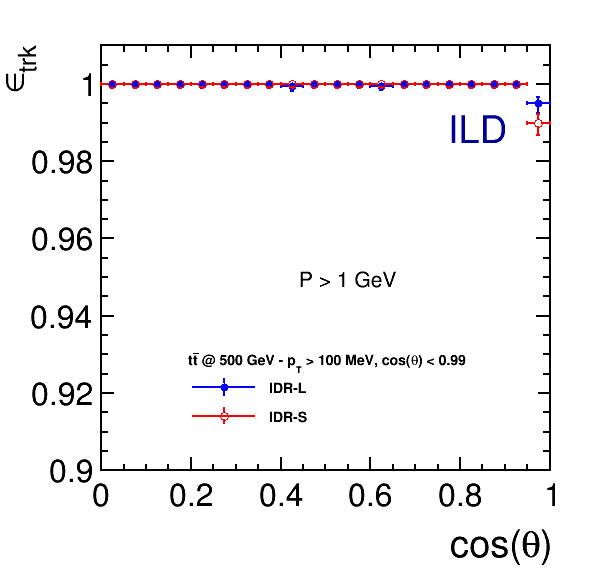
\includegraphics[width=\hsize]{Performance/fig/trkEff_th_ttbar_IDR.png}
 \caption{ \label{fig:perf:trkeff_th}}
 \end{subfigure}
\begin{subfigure}{0.49\hsize} 
 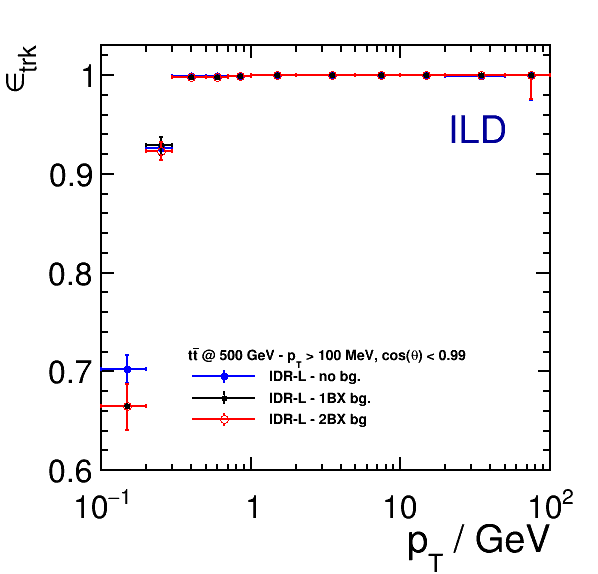
\includegraphics[width=\hsize]{Performance/fig/trkEff_pt_ttbar_pairBG_IDR.png}
 \caption{  \label{fig:perf:trkeff_bg}}
 \end{subfigure}
\begin{subfigure}{0.49\hsize} 
 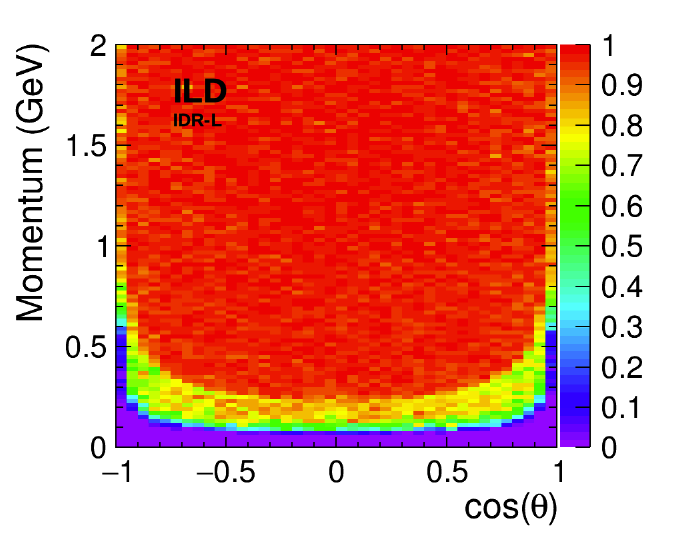
\includegraphics[width=\hsize]{Performance/fig/newSiliconTracking_10kEvents_effTrk_Momentum_v3.png}
 \caption{ \label{fig:perf:trkeff_2D_p}}
 \end{subfigure}
\begin{subfigure}{0.49\hsize} 
 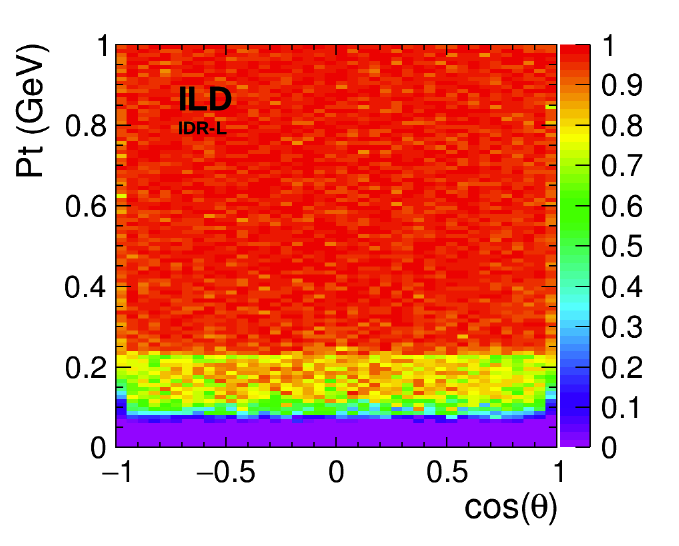
\includegraphics[width=\hsize]{Performance/fig/newSiliconTracking_10kEvents_effTrk_Pt_v3.png}
 \caption{  \label{fig:perf:trkeff_2D_pt}}
 \end{subfigure}
\caption{
  Track finding efficiency for prompt ($r_{vertex}<\unit{10}{\cm}$) tracks in $t \bar t$-events at 500 GeV as a function of kinematic variables for the large and small detector:
  (a) as a function of momentum $p$  (b) as a function of transverse momentum $p_T$ (c) as a function of $\cos(\theta)$).
  The effect on the efficiency of overlaying hits from 1BX and 2BX of pair background is shown in (d). The tracking efficiency as a
  function of $\cos(\theta)$ and either momentum or transverse momentum is shown for the large model in (e) and (f) respectively. 
}
\label{fig:perf:trkeff}
\end{figure}

The track finding efficiency of the algorithms described in section~\ref{sec:reco} is evaluated with $\Ptop\APtop$-events
at $E_{cms}=\unit{500}{\GeV}$ fully simulated and reconstructed for both detector models.
The tracking efficiency is defined as the ratio of the number of correctly reconstructed tracks with a hit purity of 75~\% to the
number of Monte Carlo tracks that are created within \unit{10}{\cm} of the {\em IP}, left at least 4 hits in the detector and
did not decay in flight. The resulting efficiency is shown in Fig.~\ref{fig:perf:trkeff} as a function of momentum $p$ in (a),
transverse momentum $p_T$ in (b) and $\cos(\theta$) in (c). As can be seen in (c), the tracking is almost perfect for particles
with $p>\unit{1}{\GeV}$ and $p_T>\unit{100}{\MeV}$ down to $\cos(\theta) \approx 0.95$ and better than 99~\% in the very forward
direction. At low momenta and in the forward direction, the small detector performs slightly worse than the larger variant, which
is due to the larger B-field that causes larger curvatures of the tracks. In the barrel region some of this effect could potentially
be alleviated by moving the innermost layer of the vertex closer to the beam, which would be possible as the background cone from
pair particles is also forced to lower radii by the higher B-field.

The qualitative dependency of the efficiency on momentum and polar angle together is shown in the 2D plots (e) and (f) for the large
detector model. The efficiency is basically flat as a function of transverse momentum in all but the very forward ($\cos(\theta)>0.95$)
part and almost perfect above $p_T>\unit{250}{\MeV}$ in that region. A small inefficiency persists in the very forward region
also for higher momenta. The above studies have been done with the same background overlaid as for the large Monte Carlo samples.
In (d) the tracking efficiency is shown also with complete and detailed simulations of one and two bunch crossings of pair
background overlaid. Only a very small degradation of the tracking efficiency at the lowest momenta is observed.

%%%%%%%%%%%%%%%%%%%%%%%%%%%%%%%%%%%%%%%%%%%%%%%%%%%%%%%%%%%%%%%
\subsection{Particle Flow performance and JER}
The performance of the Particle Flow Algorithm (PFA) is evaluated with dedicated  $\PZ\rightarrow \Pquark\APquark$-events, where
the \PZ is chosen to have the desired mass of twice the jet energy and decays at rest. This allows to distinguish the measurement of the
actual jet energy resolution (JER) from other effects like ISR-photons or confusion in jet clustering that occur in more complex,
realistic events.
%
% JER and JES for uds,c,b events
% 
\begin{figure}[htbp]
\begin{subfigure}{0.49\hsize}
 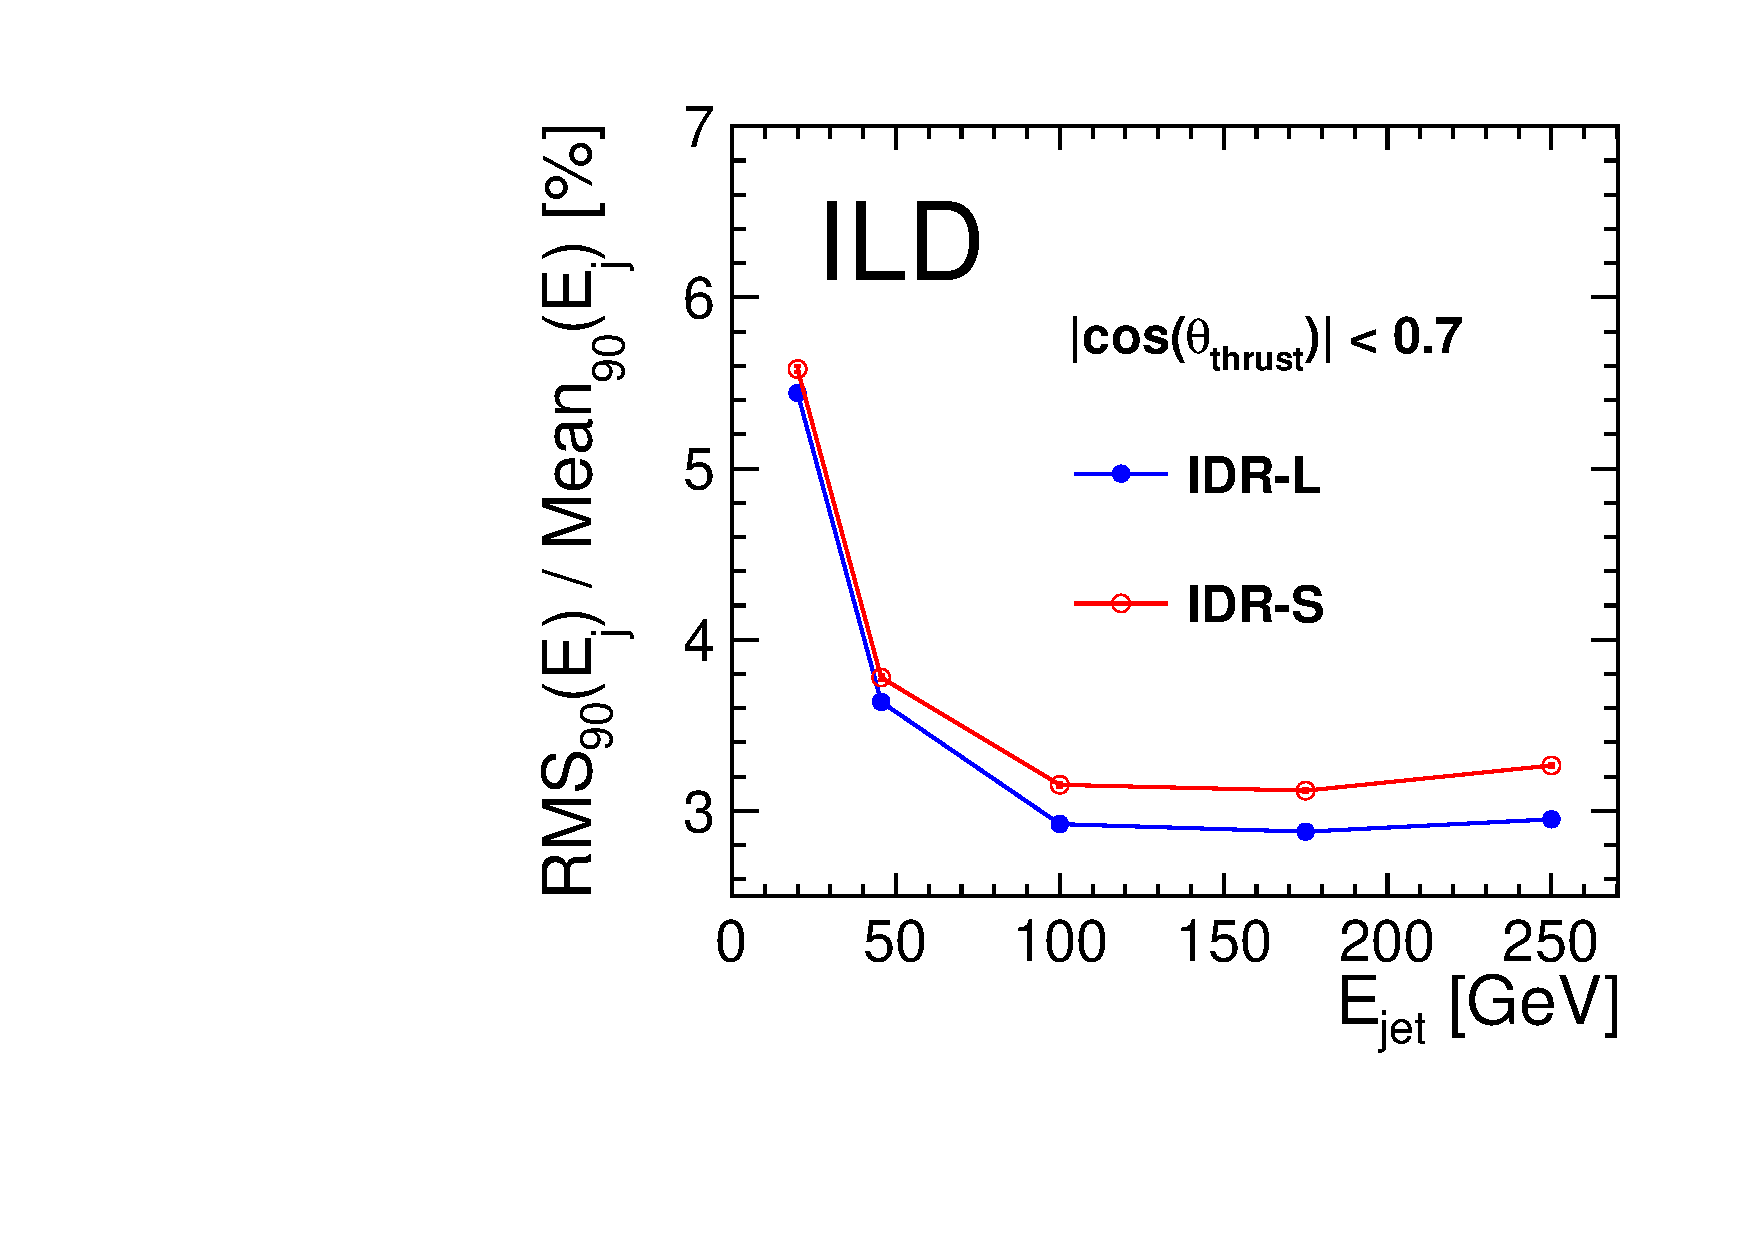
\includegraphics[width=\hsize]{Performance/fig/JERs_uds_l5_vs_s5_Barrel.pdf}
 \caption{ \label{fig:perf:pfa_jer}}
 \end{subfigure}
\begin{subfigure}{0.49\hsize}
 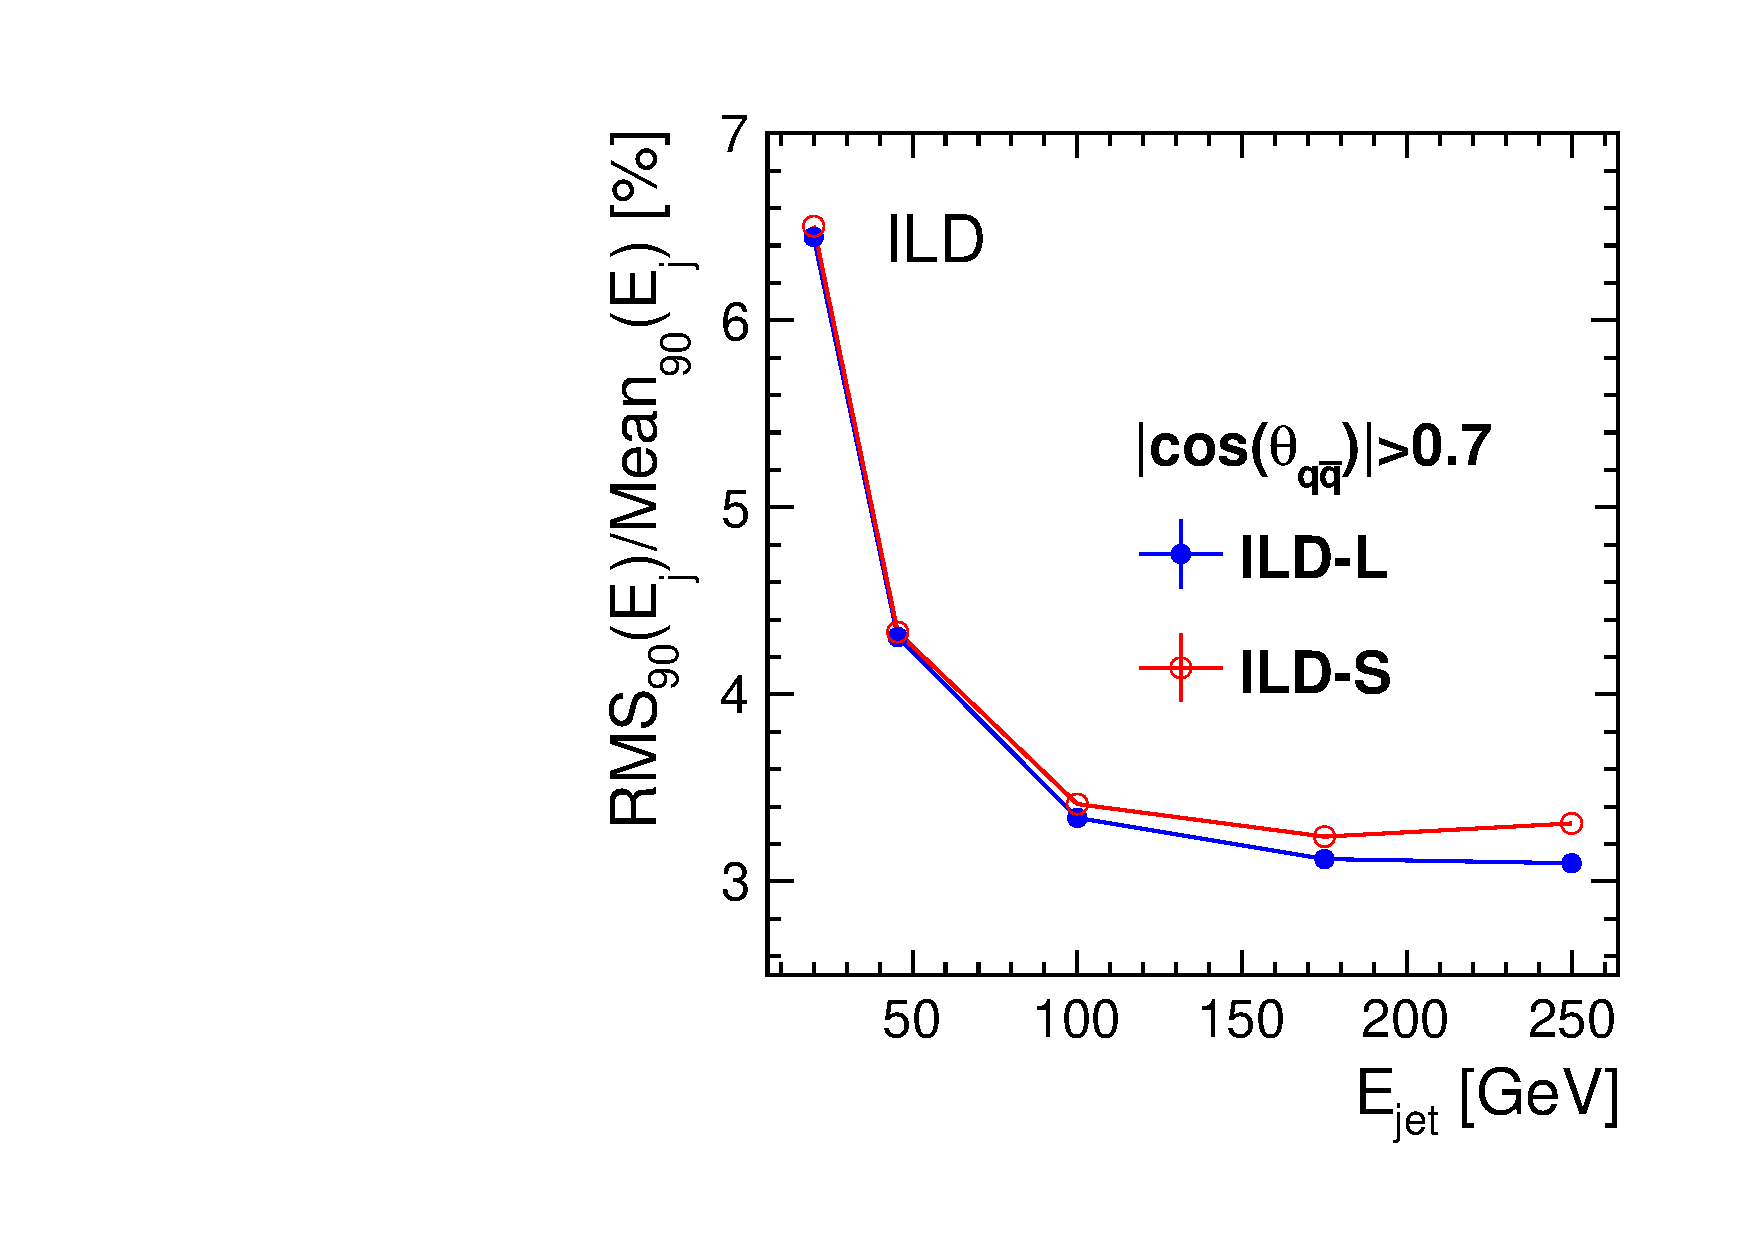
\includegraphics[width=\hsize]{Performance/fig/JERs_uds_l5_vs_s5_Endcap.pdf}
 \caption{  \label{fig:perf:pfa_jer_endcap}}
 \end{subfigure}
\begin{subfigure}{0.49\hsize}
 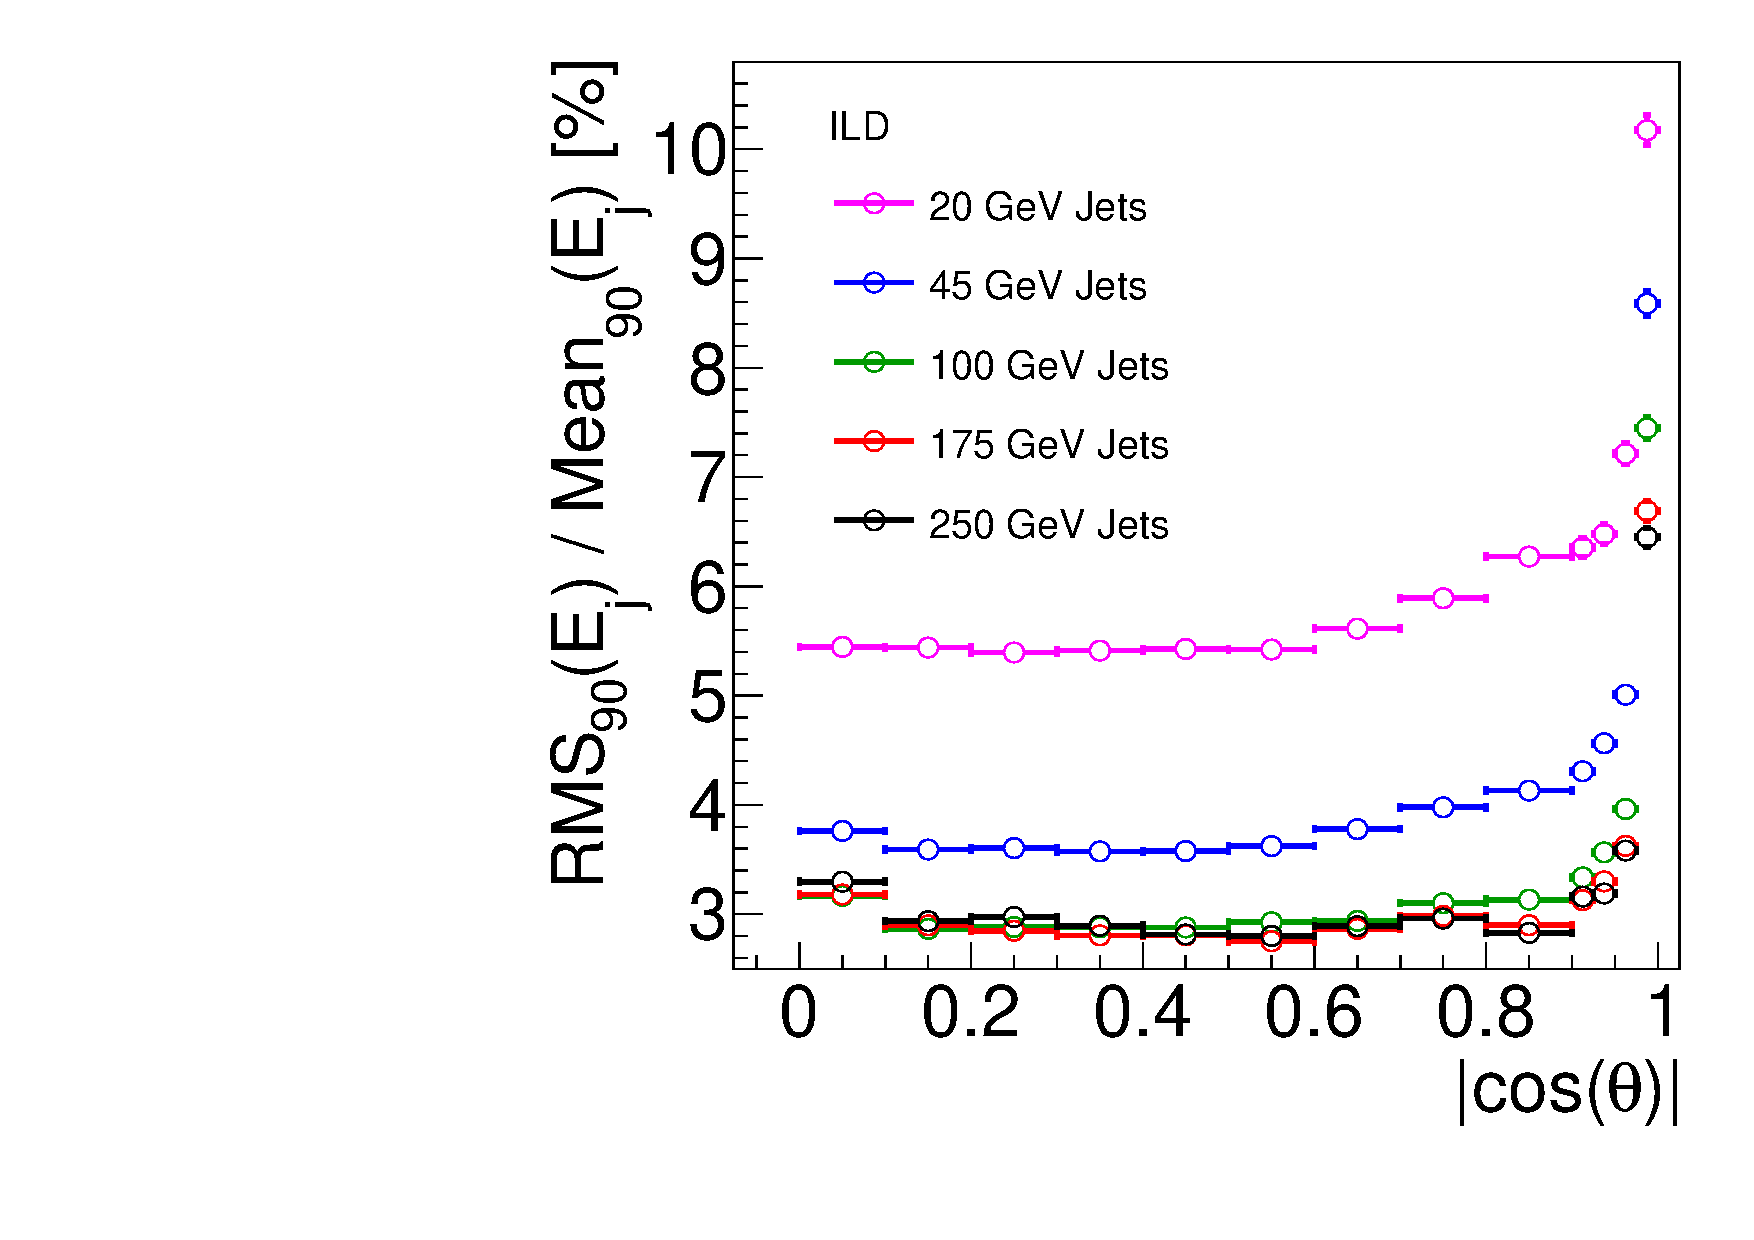
\includegraphics[width=\hsize]{Performance/fig/JER_vs_cosTheta.pdf}
 \caption{ \label{fig:perf:pfa_costh}}
 \end{subfigure}
\begin{subfigure}{0.49\hsize}
 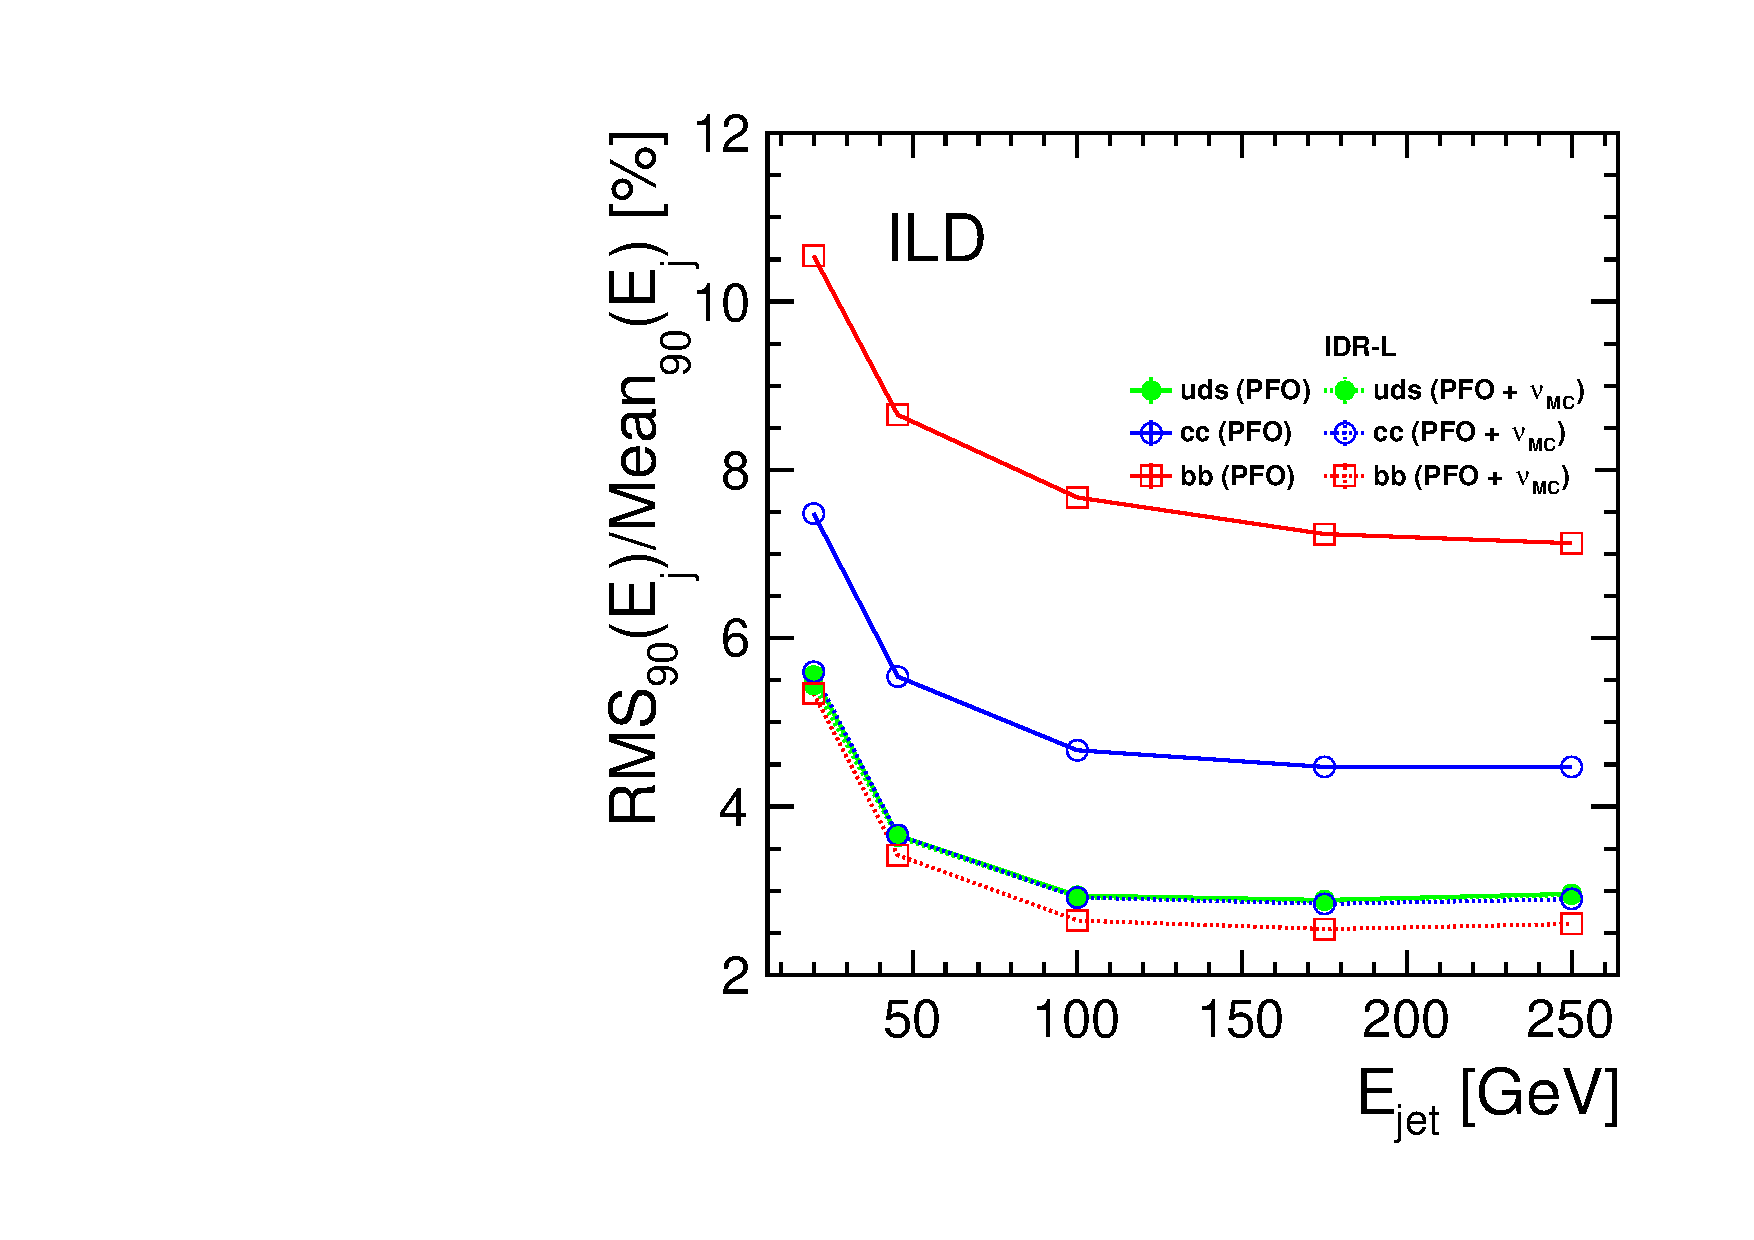
\includegraphics[width=\hsize]{Performance/fig/JERs_bcuds_pfo_vs_pfo_plus_nu.pdf}
 \caption{  \label{fig:perf:pfa_udscb}}
 \end{subfigure}
\begin{subfigure}{0.49\hsize}
 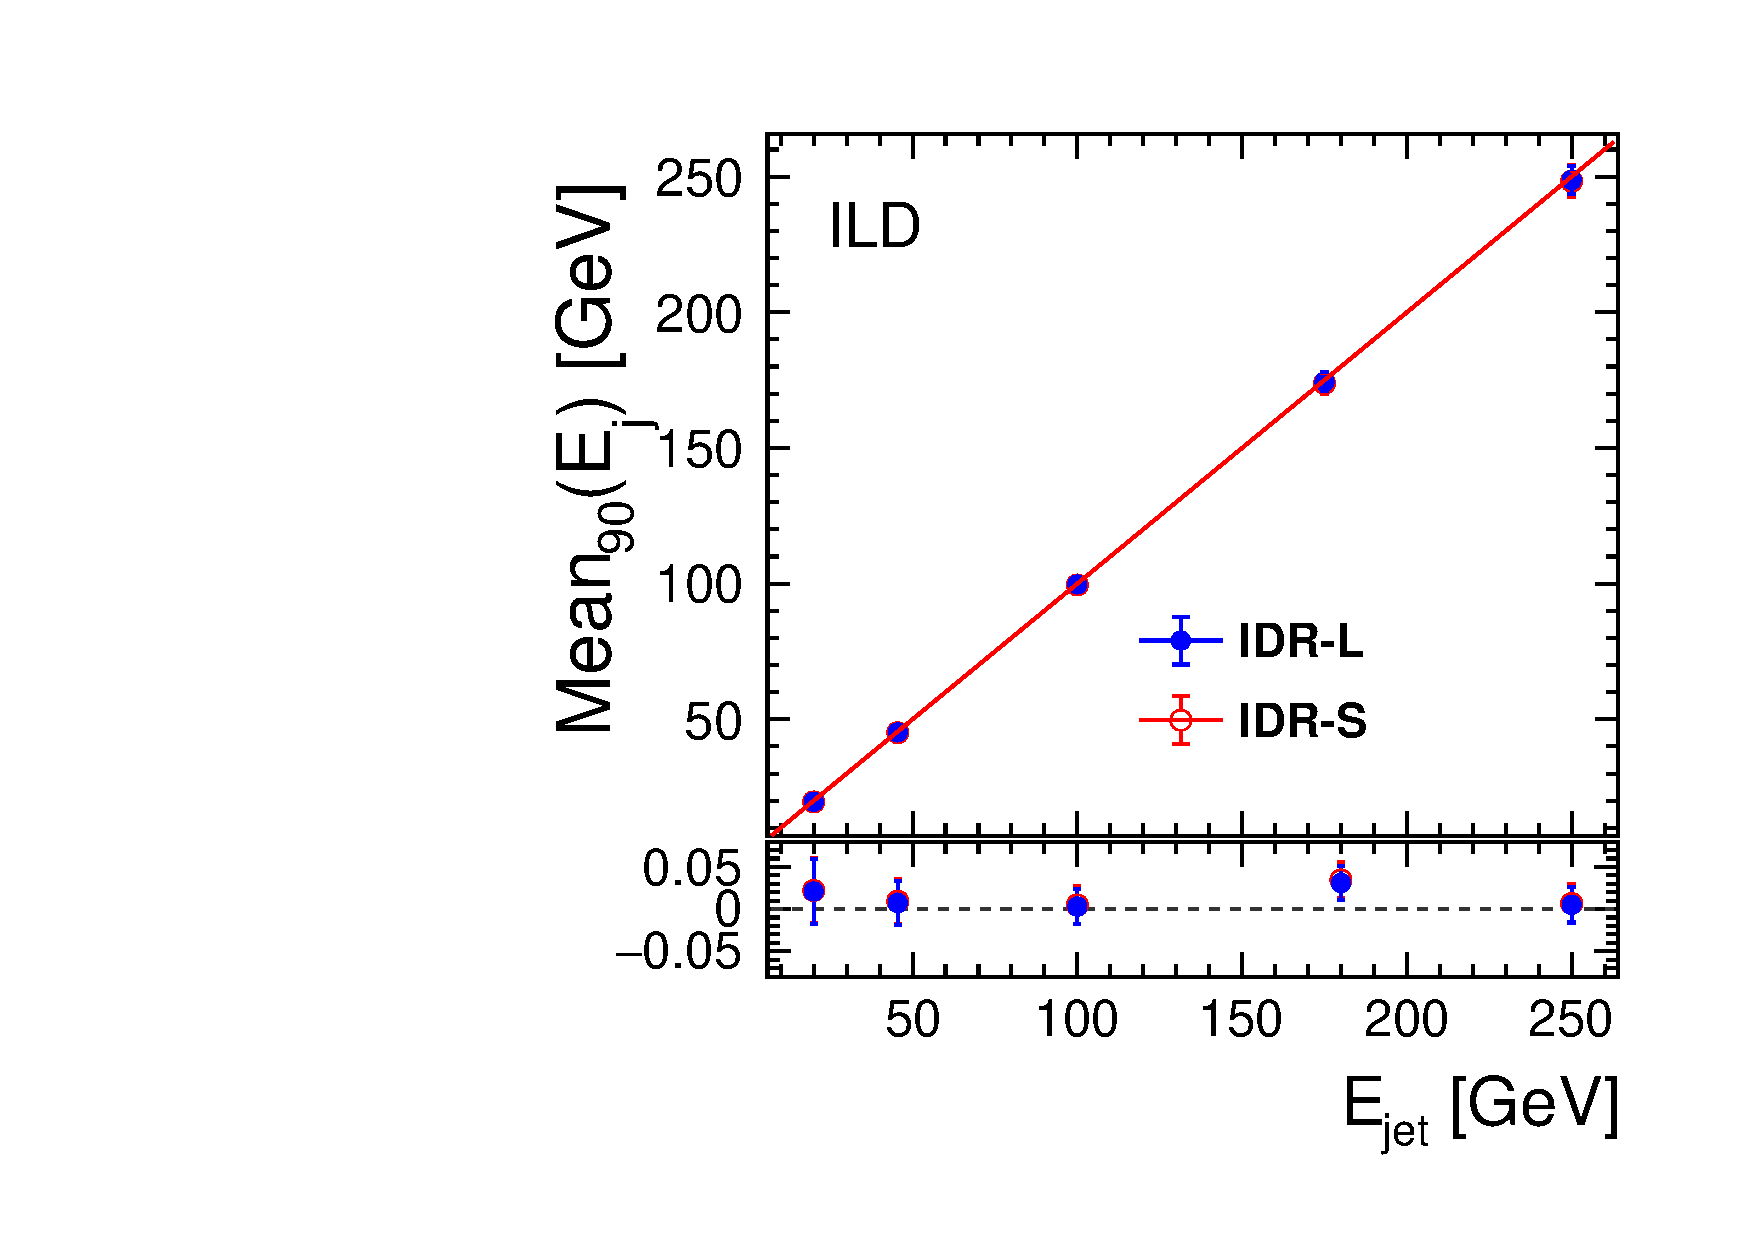
\includegraphics[width=\hsize]{Performance/fig/JESs_uds_l5_vs_s5.pdf}
 \caption{  \label{fig:perf:pfa_jes}}
 \end{subfigure}
\caption{
  Jet energy resolution (JER), evaluated as defined in eq.~\ref{ild:eq:jer} for $\PZ\rightarrow \Pquark\APquark$-events and $\Pquark \in [\Pqu,\Pqd,\Pqs]$.
  (a) comparison of the JER for the large and small ILD detector in the barrel region with
  $|\cos(\theta_{q\bar q})|<0.7$  (b) the same for the endcap region with  $|\cos(\theta_{q\bar q})|>0.7$
  (c) JER as function of the polar angle ({\em thrust}-axis) of the event. (d) JER for $\Pqu,\Pqd,\Pqs$ di-jet events together with $\Pqc\APqc$ and $\Pqb\APqb$ events,
  with (dashed lines) and without (solid lines) correcting the $\Pneutrino$ energies using Monte Carlo truth information. (e) Jet energy scale for the large and small model
  for barrel events.
  }
\label{fig:perf:pfa}
\end{figure}
%
%
The jet energy resolution is then evaluated as 
\begin{equation}\label{ild:eq:jer}
\frac{ \sigma_{E_{jet}} } { E_{jet}}  :=  \frac{\rmsn(E_{jet})}{ \mathrm{mean}_{90}(E_{jet})}
\end{equation}
for $\PZ\rightarrow \Pquark\APquark$-events with $|\cos(\theta_{q\bar q})|<0.7$ and $\Pquark \in [\Pqu,\Pqd,\Pqs]$.
The $\rmsn$ is defined to be the $rms$ of the central $90\%$ of the distribution and the $\mathrm{mean}_{90}$ is its mean value.
This measure is robust against large tails and
should be multiplied by a factor of $\sim1.1$ to obtain an equivalent Gaussian analyzing power\cite{ild:bib:PandoraPFA}.
Fig.~\ref{fig:perf:pfa_jer} shows the JER as a function of the jet energy for selected energies $E_{jet}=\unit{(20, 45, 100, 175, 250)}{\GeV}$
for the large and small detector model in the barrel region. For $E_{jet}\geq \unit{45}{\GeV}$ the resolution is better than 4\% and
approaches 3\% (3.2\%) for the large (small) model at higher energies. In the forward region ( $|\cos(\theta_{q\bar q})|<0.7$ ) the JER is
slightly worse and the difference between large and small detector is less pronounced as can bee seen in Fig.~\ref{fig:perf:pfa_jer_endcap}.
The JER as a function of the polar angle of the jets (the {\em thrust}-axis of the di-quark events) is shown in Fig.~\ref{fig:perf:pfa_costh} for the
large detector model. The observed dependency is rather flat throughout the barrel region, increasing somewhat after the barrel-end-cap transition
with a visible rise in the very forward region, similar for all energies. The effect of heavy flavor quarks on the jet energy resolution is shown in
Fig.~\ref{fig:perf:pfa_udscb}, where the resolutions is plotted for $\Pqu,\Pqd,\Pqs$ di-quark events together with $\Pqc\APqc$ and $\Pqb\APqb$ events for the large model.
The observed degradation in the JER for the heavy quark jets can be fully attributed to the missing energy carried by neutrinos,
as can be seen from the dashed lines, were the energy is corrected for the $\Pneutrino$~-energies using Monte Carlo truth information.
The linearity of the jet energy measurement is shown in Fig.~\ref{fig:perf:pfa_jes} to be better than 5\% in the barrel region.


%%%%%%%%%%%%%%%%%%%%%%%%%%%%%%%%%%%%%%%%%%%%%%%%%%%%%%%%%%%%%%%
\subsection{Vertexing}

The correct identification of heavy flavour decays in jets requires a precise measurement of the coordinates of secondary vertices.
The vertex resolution is studied using  dedicated, artificial $\Pep\Pem \rightarrow 6~\Pqc$ events, along the longitudinal direction $\vec{e}_L$
and two transverse directions $\vec{e}_{T1}$ and $\vec{e}_{T2}$, defined as:
\begin{equation}
\vec{e}_L = \frac{ \vec{p}_c }{|\vec{p}_c| }~; ~~~~~~~  \vec{e}_{T1} = \vec{e}_L \times \vec{z} ~; ~~~~~~~  \vec{e}_{T2} = \vec{e}_L \times \vec{e}_{T1}
\end{equation}
whith the 3-momentum of the $\Pqc$-quark $\vec{p}_c$.
The result is shown for the transverse (a) and longitudinal (b) components of the secondary vertices as a function of the distance from the $IP$
in Fig.~\ref{fig:perf:vtxres}.
\begin{figure}[htbp]
\begin{subfigure}{0.49\hsize}
 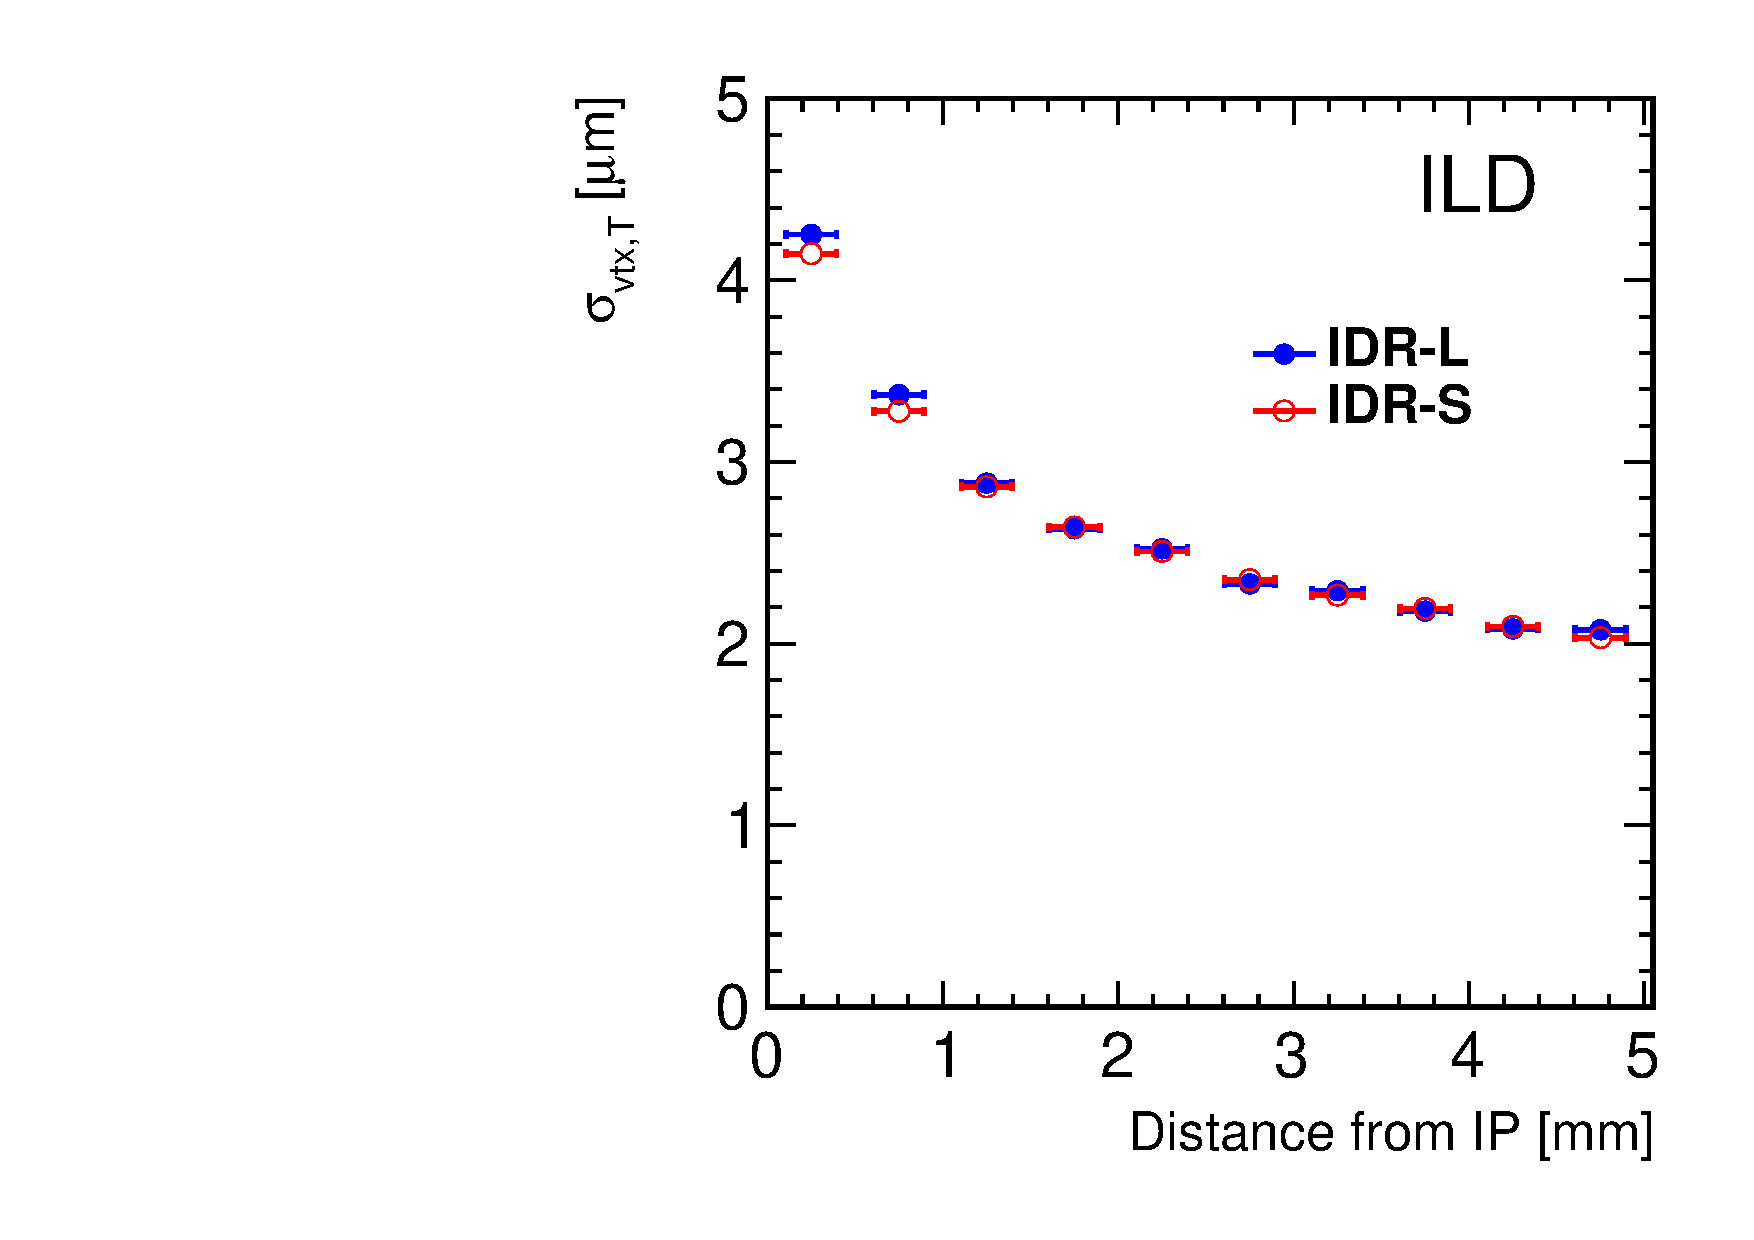
\includegraphics[width=\hsize]{Performance/fig/svtx_r_resol.pdf}
 \caption{ \label{fig:perf:svtx_r}}
 \end{subfigure}
\begin{subfigure}{0.49\hsize}
 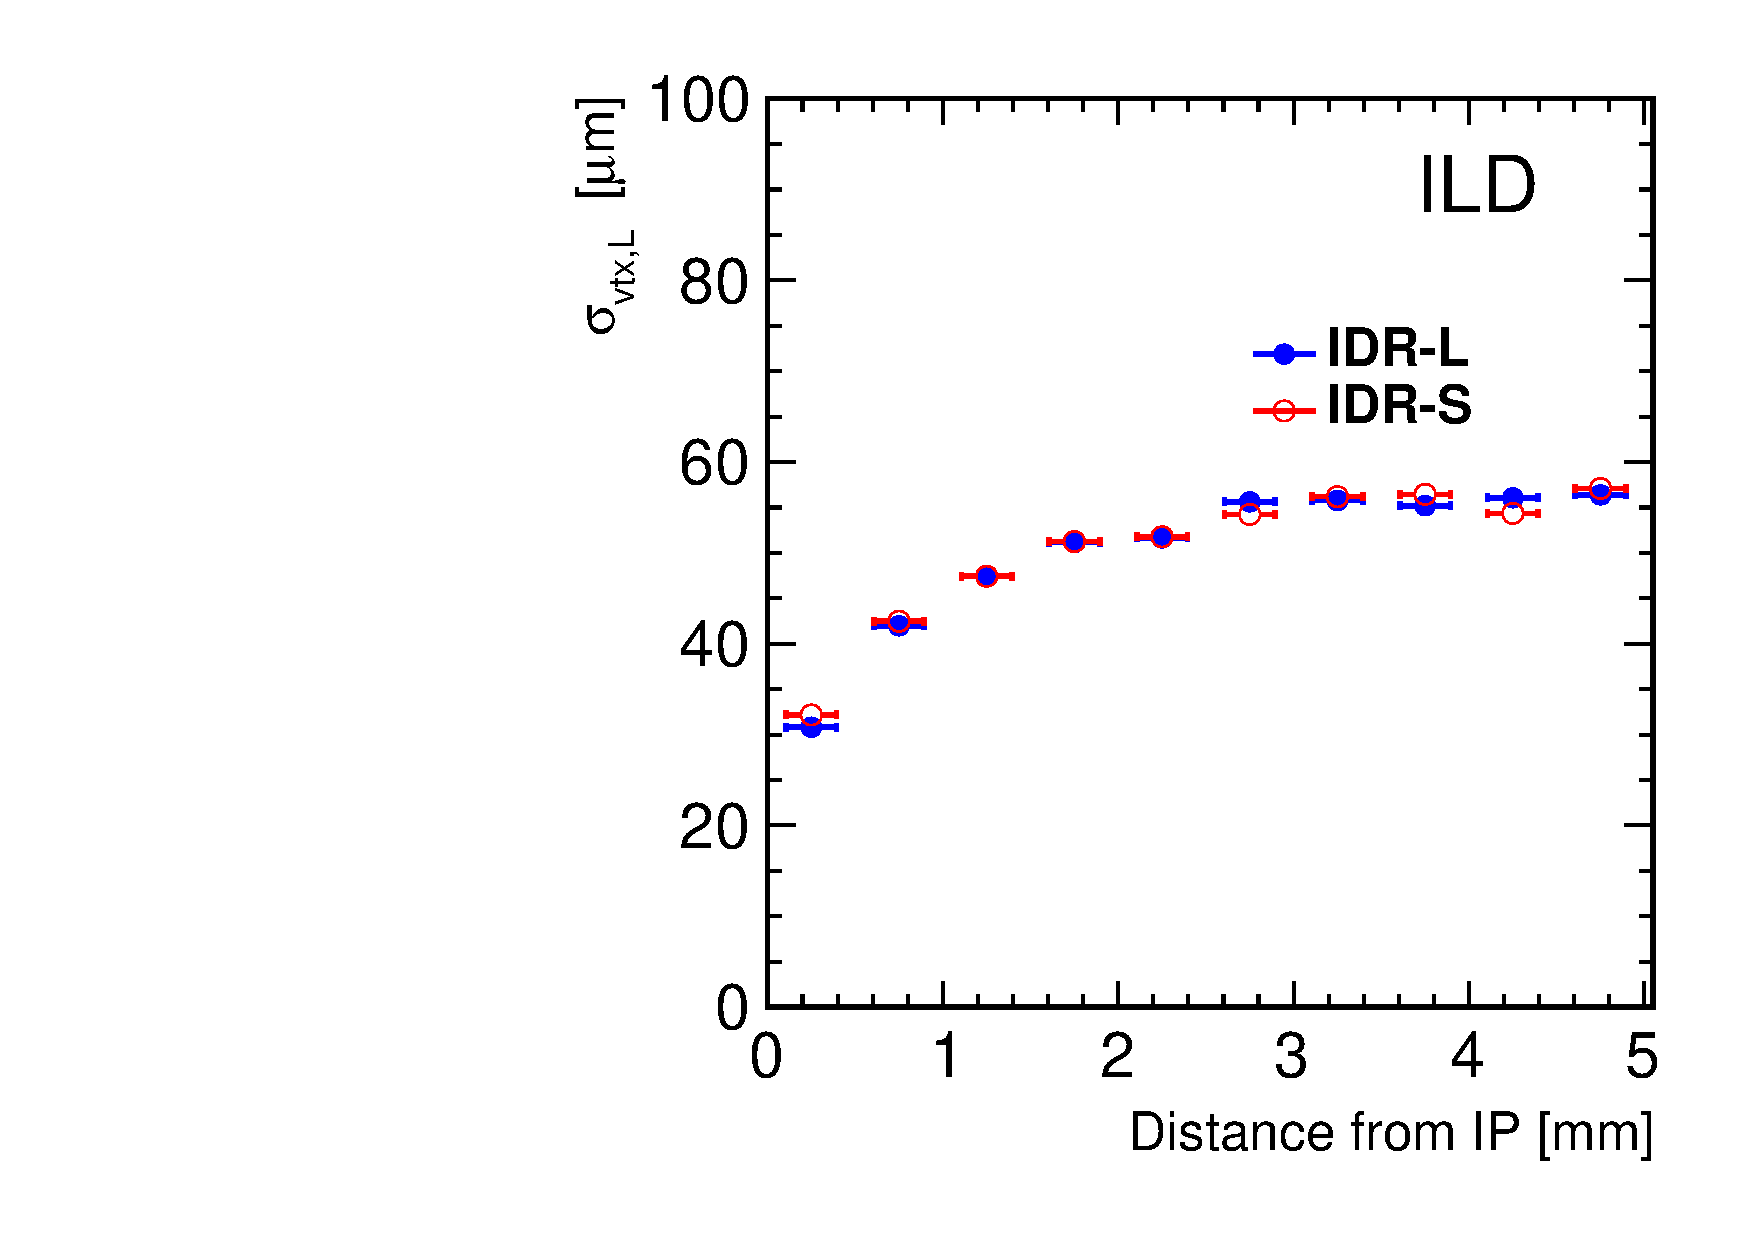
\includegraphics[width=\hsize]{Performance/fig/svtx_z_resol.pdf}
 \caption{  \label{fig:perf:svtx_z}}
 \end{subfigure}
\begin{subfigure}{0.49\hsize}
 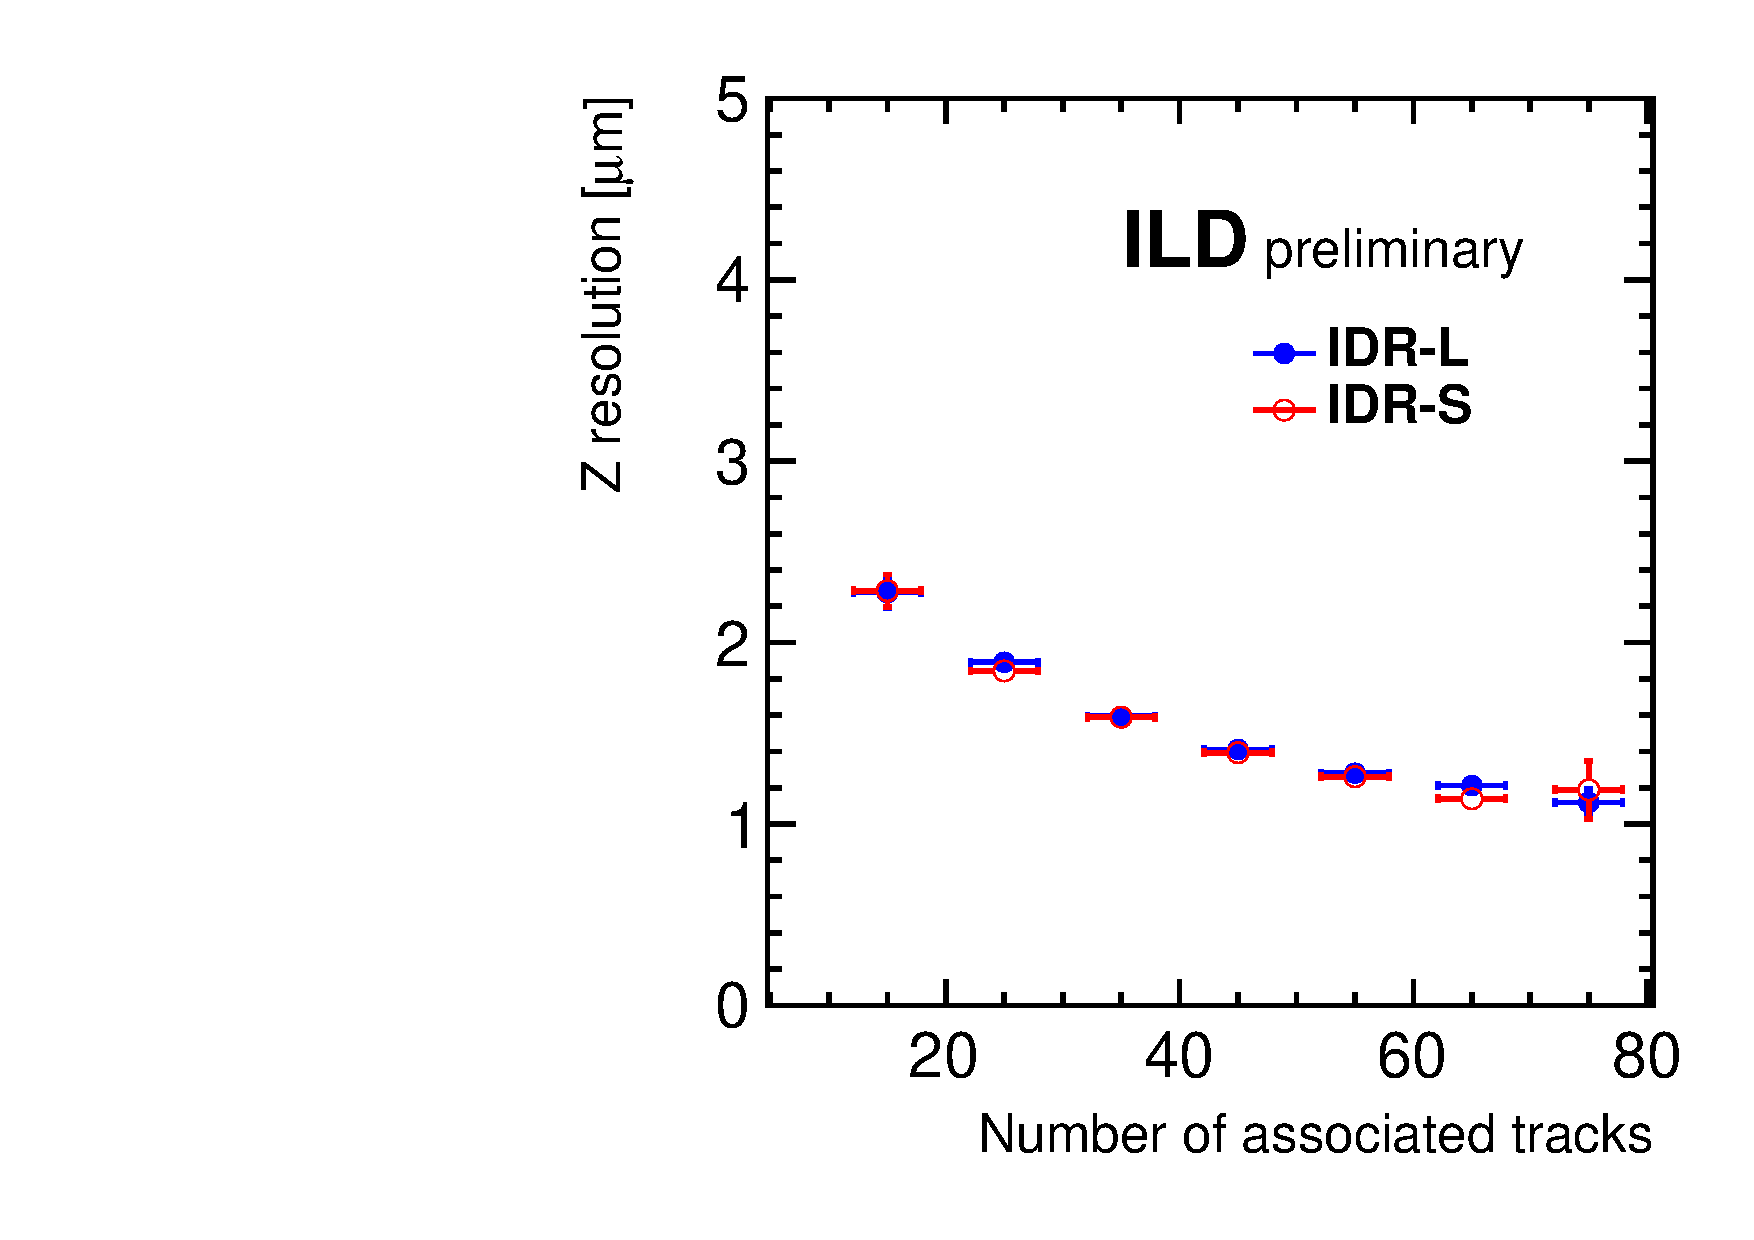
\includegraphics[width=\hsize]{Performance/fig/pvtx_z_resol.pdf}
 \caption{  \label{fig:perf:pvtx_z}}
 \end{subfigure}
\caption{ Vertex resolutions for the large and small ILD detector models.
  (a) Resolution of the transverse component of secondary vertices as a function of the distance from the $IP$ and the same for the longitudenal component in (b).
  (c) Resolution of the z-coordinate of the primary vertex as a function of the number of tracks used in the fit. 
  Note that the radial component of the primary vertex is known extremely well to \unit{O(10)}{\nm} from the beam-spot position.
}
\label{fig:perf:vtxres}
\end{figure}
%
Fig.~\ref{fig:perf:pvtx_z} shows the resolution of the primary vertex' z-position as a function of the number of associated tracks.
The resolution is better than \unit{3}{\micron} for low multiplicity events and
approaches \unit{1}{\micron} for high multiplicity events.  The radial component of the primary vertex is already known
extremely well from the beam-spot position to \unit{O(10)}{\nm}. The overall vertexing performance for the large and small detector models
is very similar, as expected already from the single track impact parameter resolutions shown in Fig.~\ref{fig:perf:trkres} (c)-(f).



%%%%%%%%%%%%%%%%%%%%%%%%%%%%%%%%%%%%%%%%%%%%%%%%%%%%%%%%%%%%%%%
%%\subsection{Photon Reconstruction}
%%\fix{no publishable results for photon ID available ...}
%%%%%%%%%%%%%%%%%%%%%%%%%%%%%%%%%%%%%%%%%%%%%%%%%%%%%%%%%%%%%%% 
%%\subsection{Lepton ID}
%%\fix{muons, electrons - no publishable results for lepton ID available ...}
%%%%%%%%%%%%%%%%%%%%%%%%%%%%%%%%%%%%%%%%%%%%%%%%%%%%%%%%%%%%%%%
\subsection{Charged Particle identification}
%\fix{dE/dx, potentially ToF, shower shapes}
%
%
Measuring the energy loss of charged particles in the ILD-TPC provides powerful tool for identifying the type of the particle.
\thisfloatsetup{floatwidth=\SfigwFull,capposition=beside}
\begin{figure}[b!]
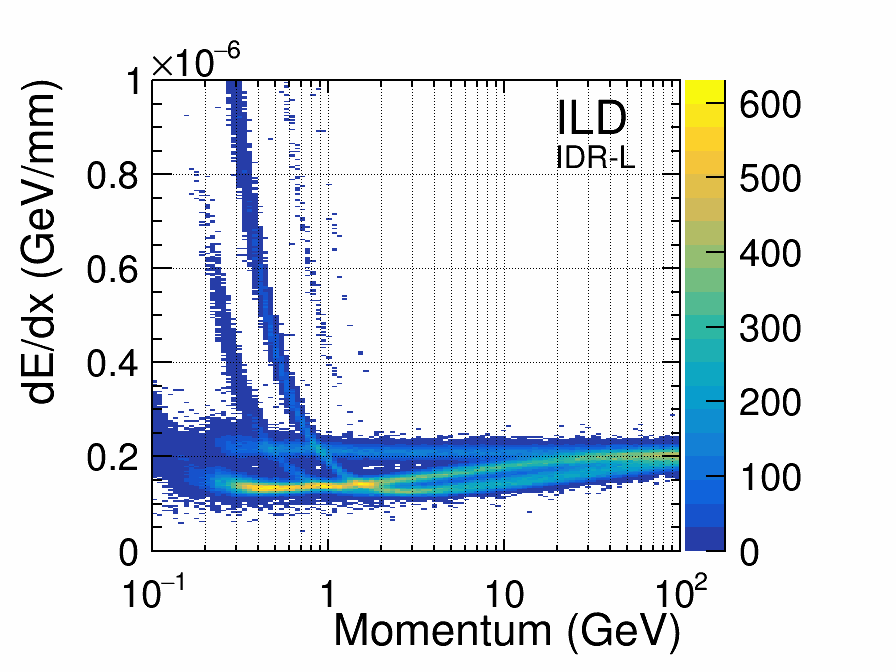
\includegraphics[width=0.8\hsize]{Performance/fig/dEdx_BBAll_lowGran_bigCap.png}
\caption{\label{fig:perf:dedx_tpc}
  $dE/dx$ as a function of particle momentum as reconstructed from a full simulation of particles in the TPC of the large detector model.
}
\end{figure}
%
Fig.~\ref{fig:perf:dedx_tpc} shows the $dE/dx$ reconstructed from a truncated mean for charged particle tracks in the TPC as a function of
the particle momentum, clearly revealing the bands of the most abundant particle types $\Pepm, \Pmupm, \Ppipm, \PKpm$ and $\Pproton$.
By fitting Gaussian distributions, with mean $\mu(p)$ and standard deviation $\sigma(p)$, to individual bands in momentum bins one can
define a separation power $\eta_{A,B}$ for distinguishing the two particle types A and B:
\begin{equation}
\eta_{A,B}(p) = \frac{ |\mu_A(p) - \mu_B(p)| } { \sqrt{ \frac{1}{2} ( \sigma^2_A(p) + \sigma^2_B(p) )  }  }
\label{ild:eq:seppow}
\end{equation}
Figure~\ref{fig:perf:dedxtof} shows the separation power
for $\Ppi,\PK$ and $\PK,\Pp$  based on the $dE/dx$ measurement in the TPC of the large and small detector model (a)
and the possible improvement that could be achieved by combining it with a  {\em time-of-flight (TOF)} measurement in the large detector (b).
As a proof of concept a possible TOF estimator is computed here. It uses the first ten calorimeter hits in the Ecal that are closest to the straight line,
resulting from extrapolation of the particle's momentum into the calorimeter, assuming an individual time resolution of $100$~ps
per hit\footnote{While this time resolution seems realisticly possible, it has to be noted, that so far it has not yet been demonstrated
 in a test beam prototype.}. The results optained clearly motivate further studies on timing measurements and optimised TOF estimators
in the ILD calorimeters.
%
% dE/dx separation power - combined w/ TOF
% 
\begin{figure}[htbp]
\begin{subfigure}{0.49\hsize}
 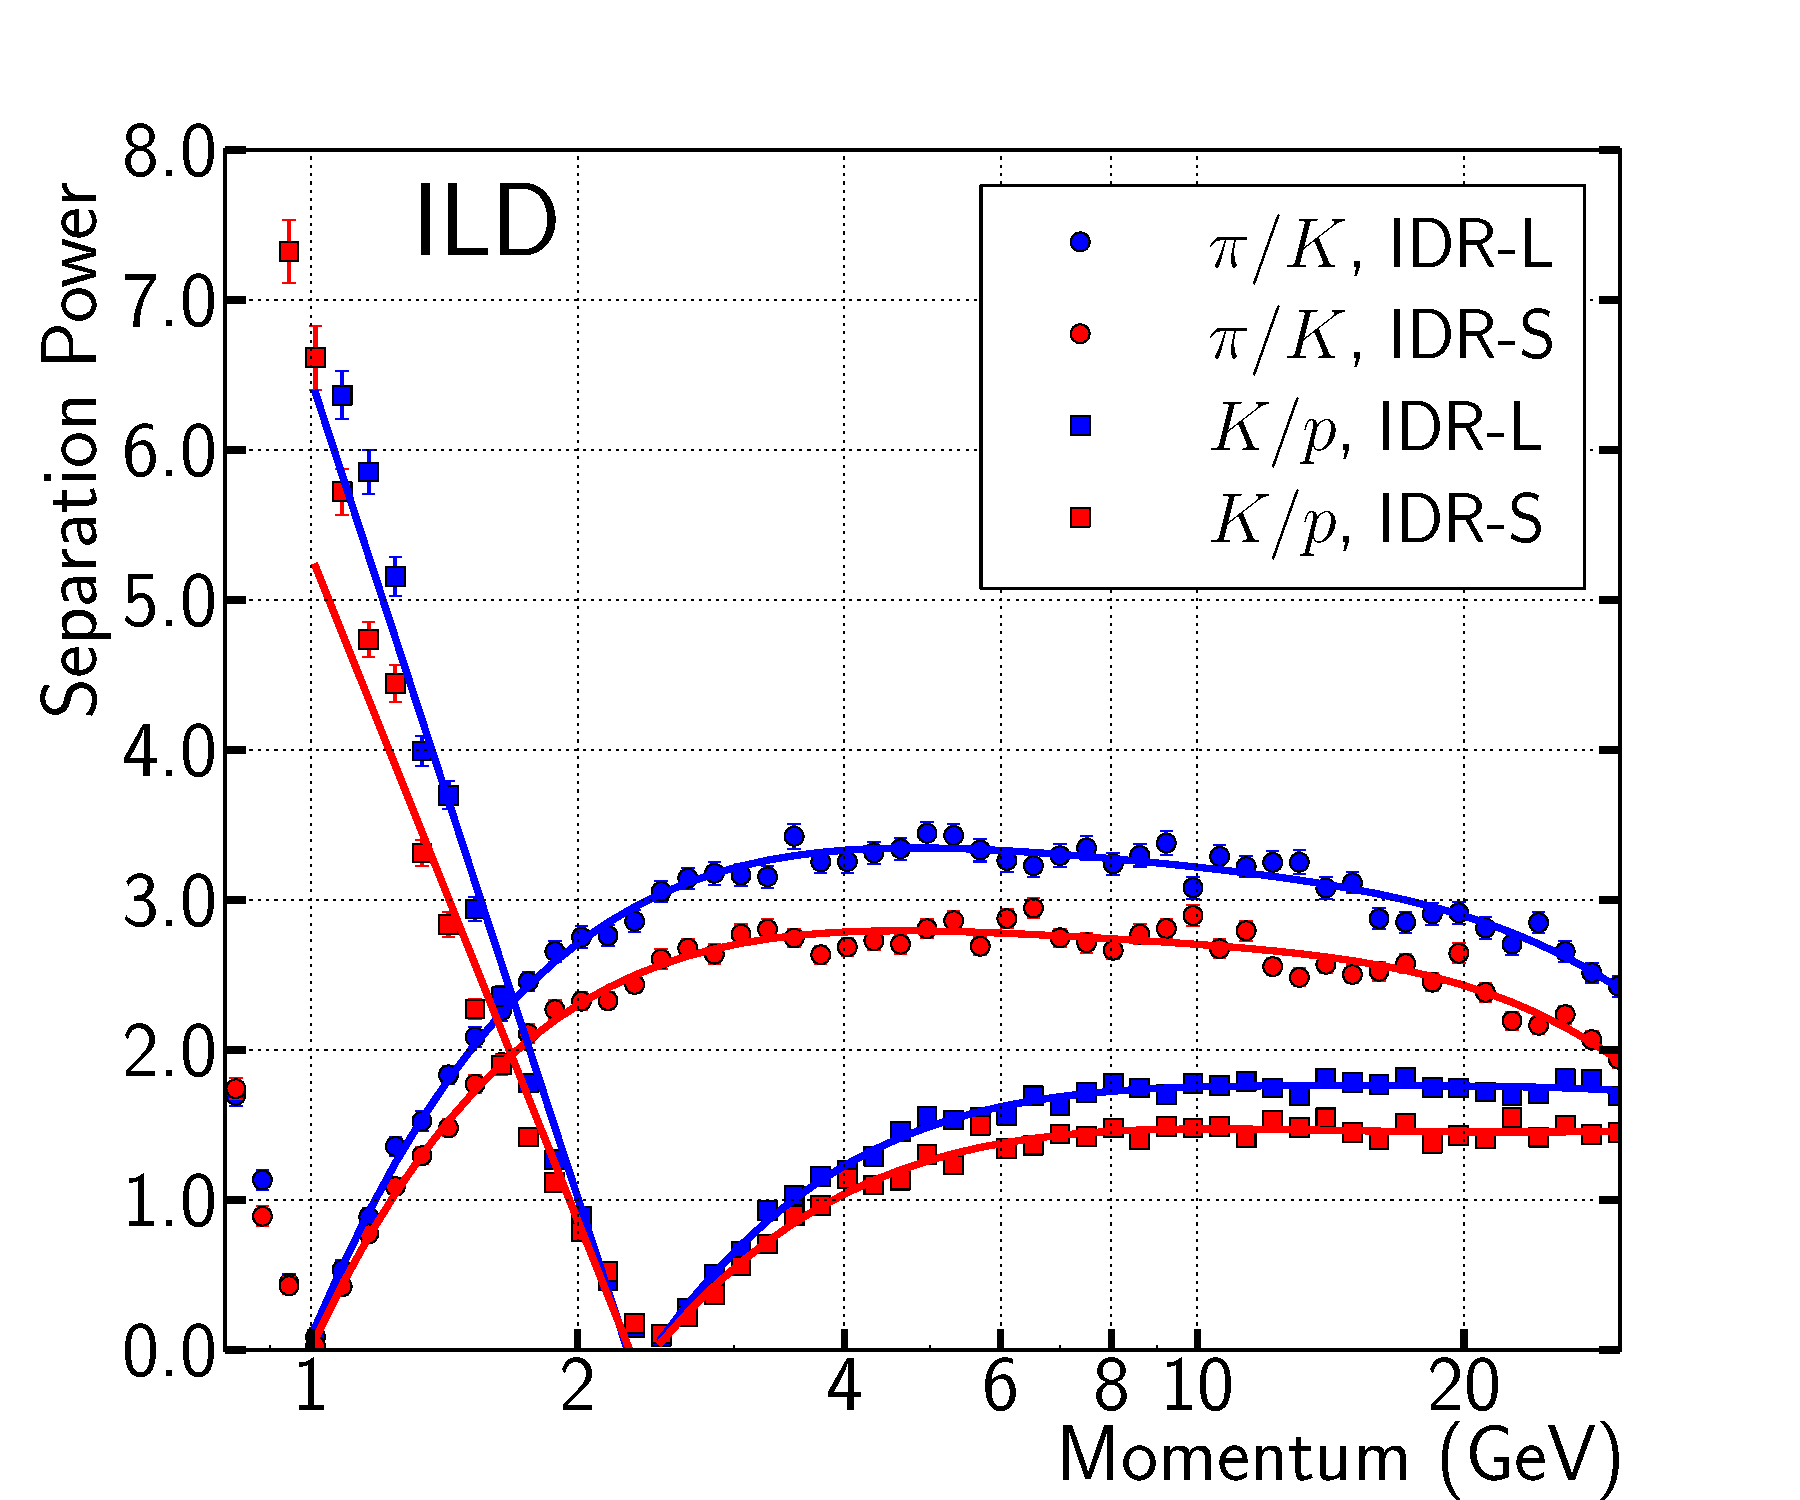
\includegraphics[width=\hsize]{Performance/fig/dEdx_ILDls_separation_power.pdf}
 \caption{ \label{fig:perf:dedx_sep}}
 \end{subfigure}
\begin{subfigure}{0.49\hsize}
 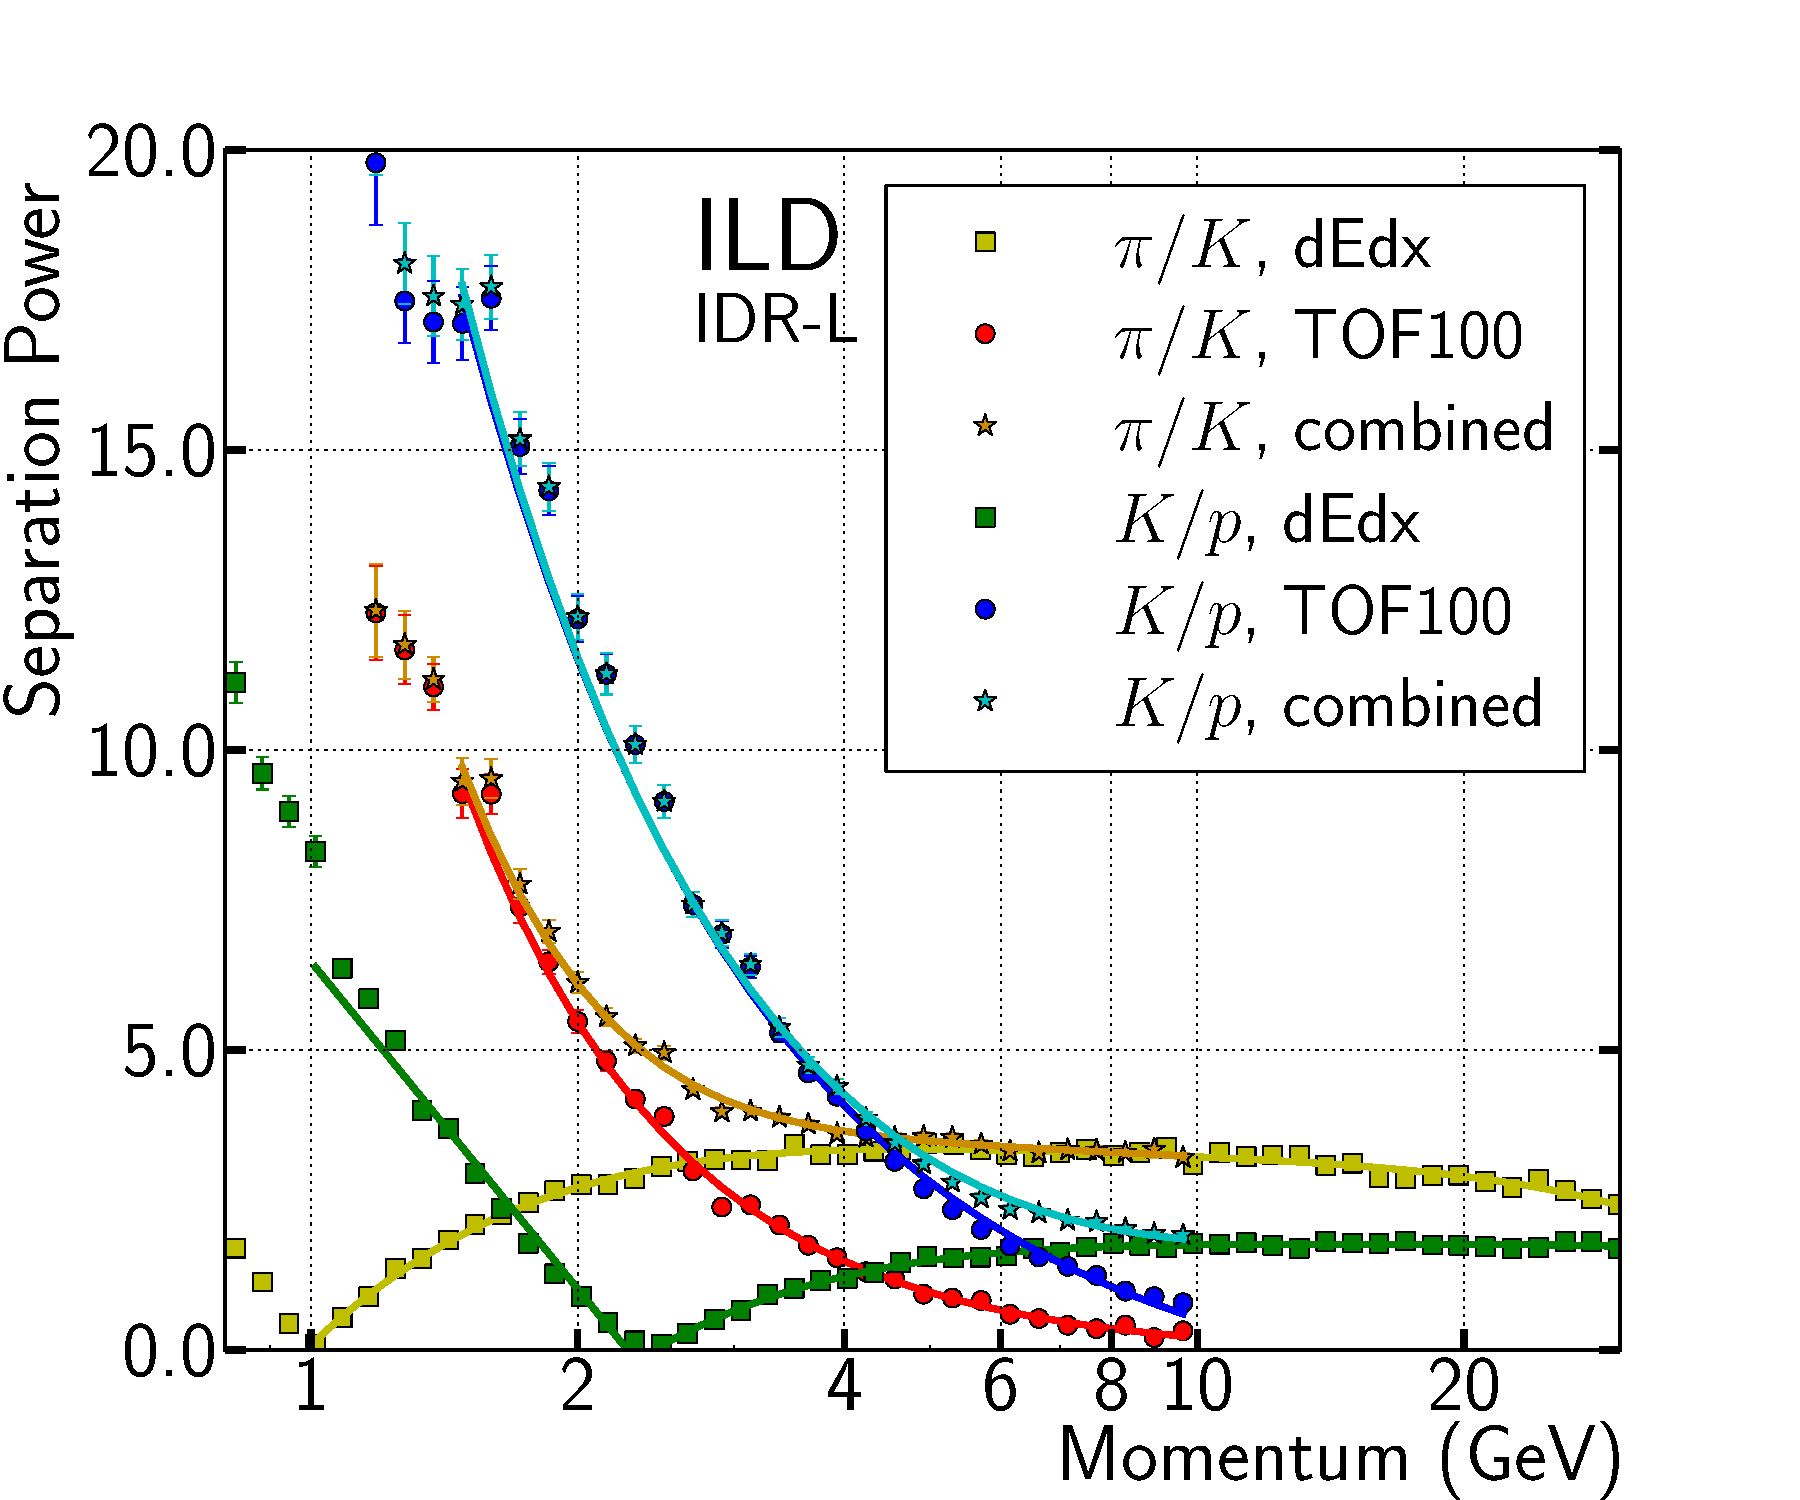
\includegraphics[width=\hsize]{Performance/fig/Combined_dEdx_TOF100_HiStat.pdf}
 \caption{  \label{fig:perf:dedxtof_sep}}
 \end{subfigure}
\caption{ (a) particle separation power (eq.~\ref{ild:eq:seppow}) for $\Ppi/\PK$ and $\PK/\Pp$ based on the $dE/dx$ measurement in the TPC.
  (b) improvement of the same separation power if combined with a {\em time-of-flight (TOF)} estimator from the first ten Ecal layers,
  where $\eta_{dE/dx,TOF}=\eta_{dE/dx} \oplus \eta_{TOF}$.
}
\label{fig:perf:dedxtof}
\end{figure}

An example in the context of physics analyses can be seen in Fig.~\ref{fig:perf:KaonID}. It compares the performance of the charged Kaon identification based on $dE/dx$ for the large and small detector models, as obtained from the $b\bar{b}$ and $t\bar{t}$ benchmarks described in Sec.~\ref{subsec:bench:bbbar} and~\ref{subsec:bench:ttbar}, respectively. For the same efficiency, the large detector reaches a $5\%$ higher purity due to its larger TPC radius, which results in a better $dE/dx$ resolution.
\thisfloatsetup{floatwidth=\SfigwFull,capposition=beside}
\begin{figure}[b!]
  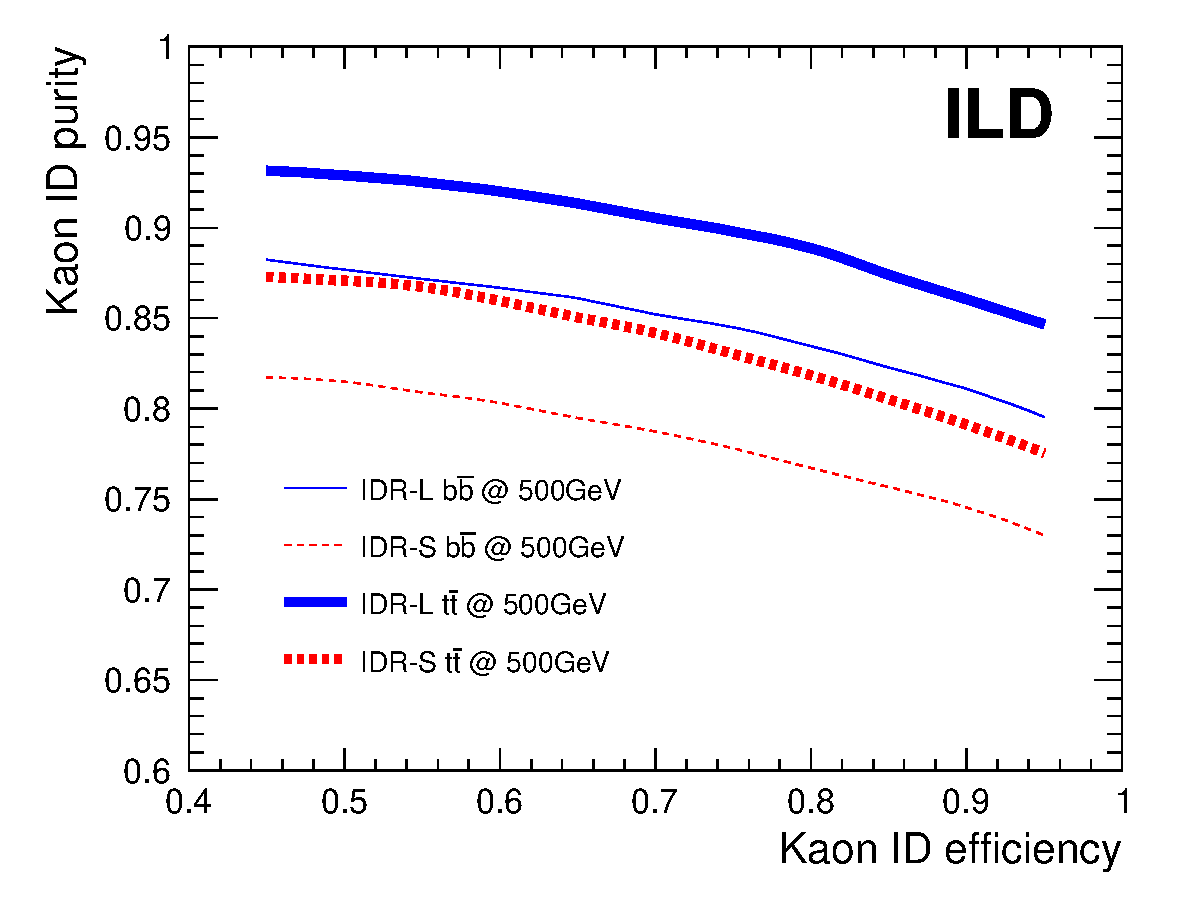
\includegraphics[width=0.8\hsize]{Performance/fig/kaonIDeff_v2-eps-converted-to.pdf}
  \caption{\label{fig:perf:KaonID}
    Efficiency-purity curves for charged Kaon identification in the context of the $t\bar{t}$ and $b\bar{b}$ analyses. For the same
    efficiency, the large detector reaches a $5\%$ higher purity due to its larger number of TPC measurements, which results in a better $dE/dx$
    resolution. Details on the analyses can be found in Sec.~\ref{subsec:bench:bbbar} and~\ref{subsec:bench:ttbar}.
  }
\end{figure}
Additional methods for charged particle identification using calorimeter shower shapes have been developed and used in specific physics analyses~\fix{[need references...]}


%%%%%%%%%%%%%%%%%%%%%%%%%%%%%%%%%%%%%%%%%%%%%%%%%%%%%%%%%%%%%%%
\subsection{BeamCal reconstruction}

Many analyses require the efficient measurement of electromagnetic showers at small polar angles in the BeamCal.
Due to the large amounts of background from pair particles (c.f.~\ref{sec:beam:background}), the BeamCal requires a special reconstruction algorithm
for identifying showers in the presence of background.
Fig.~\ref{fig:perf:beamcal_eff} shows the achieved reconstruction efficiency for single \unit{30}{\GeV} photons for the large and small detector models
for $E_{cms}=\unit{500}{\GeV}$  and $E_{cms}=\unit{250}{\GeV}$ respectively. Due to the significantly larger backgrounds at \unit{500}{\GeV} the efficiency
rises slower with polar angle than at \unit{250}{\GeV} and there is almost no difference observed between the two models.
In contrast at lower center of mass energy the small detector shows better performance, as expected due to the reduced background as an effect of the
higher B-field. Here a plateau of the efficiency at $\approx 80\%$~is reached between \unit{15}{\mrad} and \unit{20}{\mrad} due to the keyhole opening
of the BeamCal front face.
Fig.~\ref{fig:perf:beamcal_fake} shows the fraction of events where ... \fix{need updated plot and proper definition of what is plotted here ...}
%
% BeamCal Reco for single electrons
%
\begin{figure}[htbp]
\begin{subfigure}{0.49\hsize}
 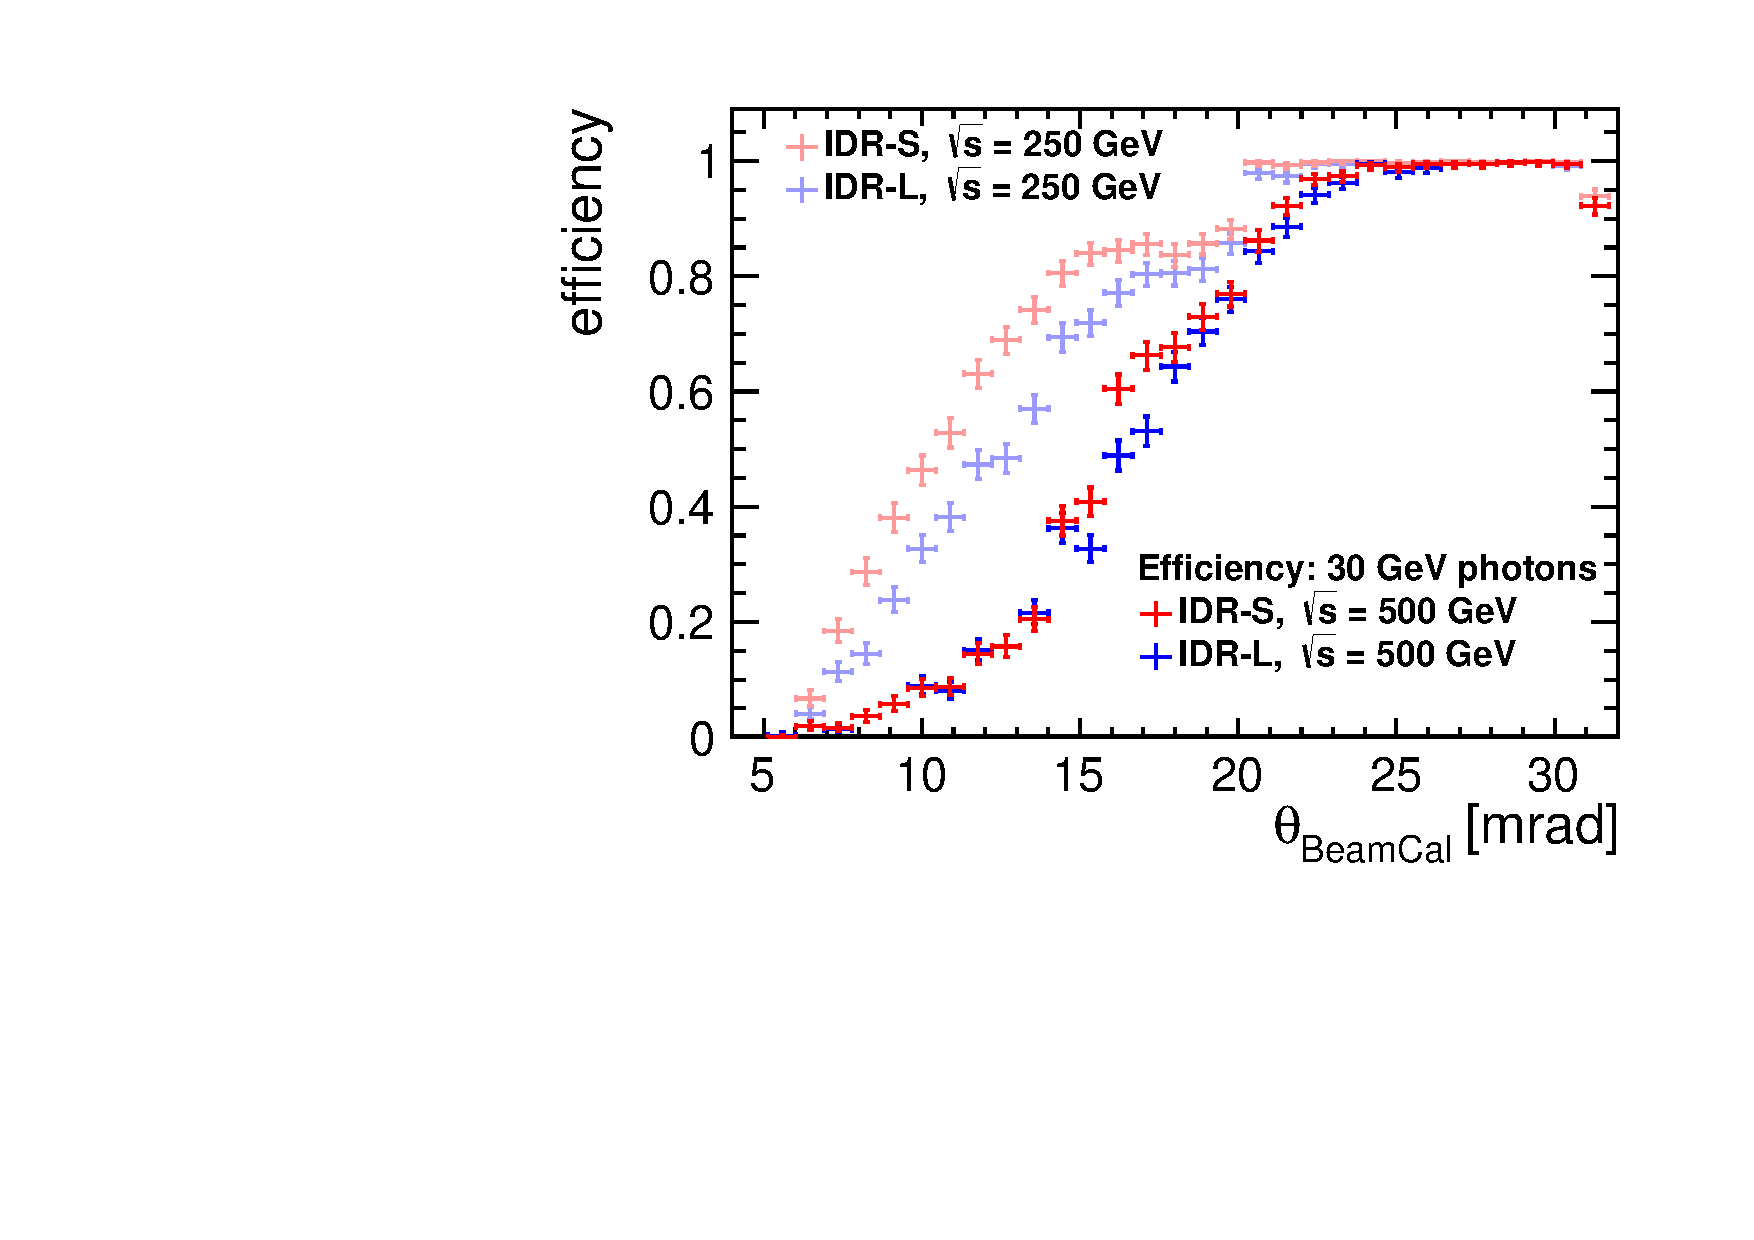
\includegraphics[width=\hsize]{Performance/fig/Eff_30GeVPhotons_different_detectors_differentCOMenergies.pdf}
 \caption{ \label{fig:perf:beamcal_eff}}
 \end{subfigure}
\begin{subfigure}{0.49\hsize}
 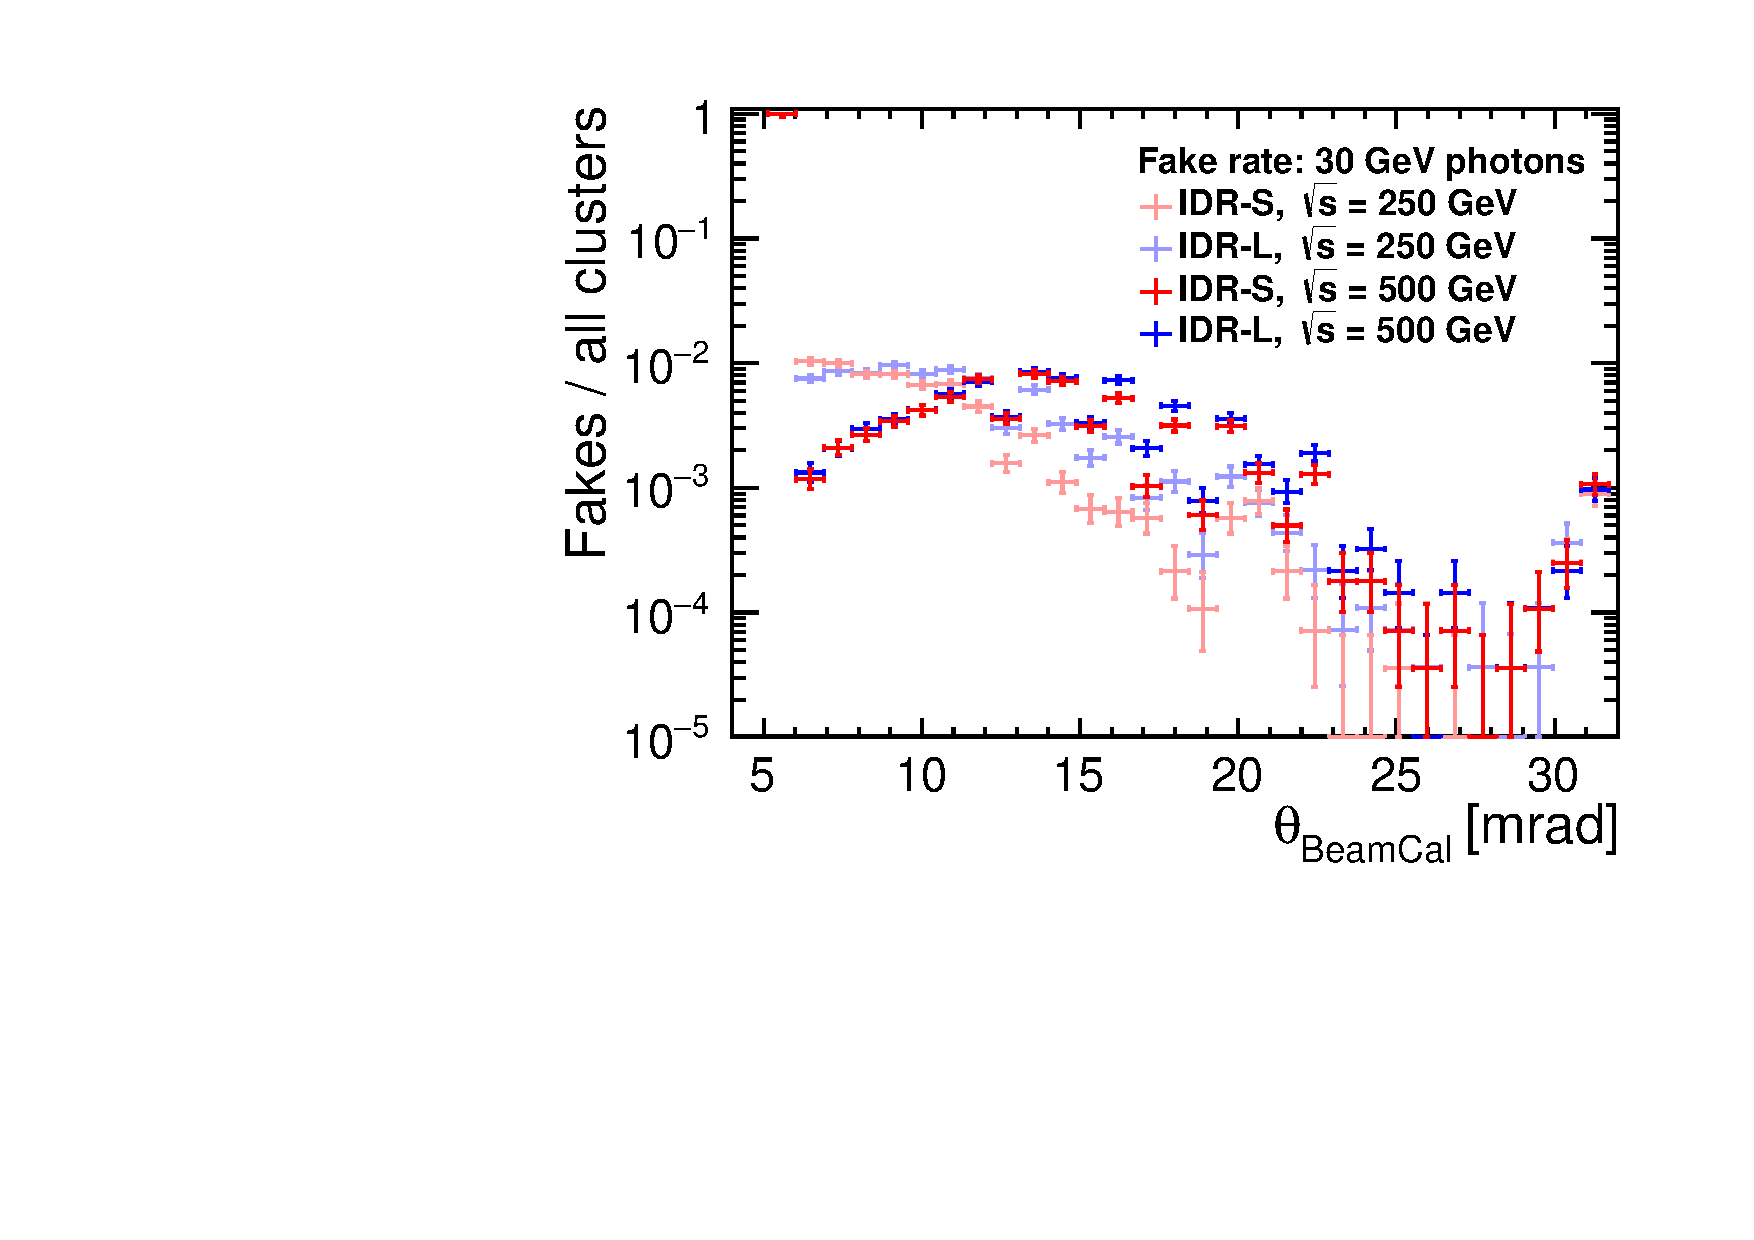
\includegraphics[width=\hsize]{Performance/fig/Fakes_30GeVPhotons_different_detectors_differentCOMenergies.pdf}
 \caption{  \label{fig:perf:beamcal_fake}}
 \end{subfigure}
\caption{ (a) Reconstruction efficiency for single \unit{30}{\GeV} photons in the large and small detector models for $E_{cms}=\unit{500}{\GeV}$  and
  $E_{cms}=\unit{250}{\GeV}$.
  (b)  Fake rate ...  1-purity ... \fix{need updated plot and proper definition of what is plotted here ...}
}
\label{fig:perf:beamcal}
\end{figure}
